\part{Managing the Lifetime of Data}

\begin{comment}
chapter 1: basics of lifetime patterns
chapter 2: aside for basics of memory management
chapter 3: time-space tradeoffs (optimization)
chapter 4: basics+optimizations -> requiremnts; how to implement these things
chapter 5: out of the box




feasibly recomputable state
for recomputable, either recompute every time, recompute some times, recompute
never

sharing pool; flyweight; shared immutable factory pattern (coding pattern)

inmemory designs; time-space tradeoffs; correlated lifetime

three risks: introduce leaks, create concurrency problems, extra space
consumption

\end{comment}

\chapter{Lifetime Requirements}
\index{Lifetime Requirements}

Your application needs some objects to live forever and it needs the rest to die
a timely death. Unfortunately, some of the important details governing memory
management are left in your hands. Java promised, with its automatic memory
management, that you could create objects without regard for the messy details of
storage allocation and reclamation. In Java, you needn't explicitly free objects,
which is at once the saviour from, and the source of, many problems with memory
consumption. Unless you are careful, your program will suffer from bugs such as
memory leaks\index{Memory Leaks}, race conditions, lock contention, or excessive
peak footprint. Furthermore, if your objects don't easily fit into the limits of
a single Java process, you will need to manage, explicitly, marshalling them in
and out of the Java heap.\index{Marshalling}

Very often, your application uses a data structure in a way that falls into one
of a handful of common \emph{lifetime requirements}\index{Lifetime Requirements}. The
nature of each requirement dictates how much help you will get from the Java runtime
in the desired preservation and reclamaion of objects, and where it leaves you to
your own devices. 

An important step in the design process of any large application is understanding
the lifetime requirement for each of your data models. In this chapter, we
describe the five common lifetime requirements: objects needed only transiently,
objects needed for the duration of the run, objects whose lifetime ends along
with a method invocation, objects whose lifetime is tied to some other object,
and, most difficult of all, objects that live or die based on need.
\autoref{tab:five-lifetimes} summarizes these five important requirements. We step
you through each of the requirements, defining them and giving examples of how to
know when you have an instance of each.

\begin{table}
\centering
%	\begin{tabular}{lp{0.30\textwidth}p{0.35\textwidth}}
	\begin{tabular}{ll}
	\toprule
	  %&
	   Lifetime Requirement & Example \\ \cmidrule(r){1-1} \cmidrule(l){2-2}
	   %\cmidrule(r){2-2} \cmidrule(l){3-3}
	%\autoref{temporary-lifetime} &
	  Temporary & new parser for every date
	\\
	%\autoref{correlated-lifetime} &
	Correlated with Another Object & object annotations
	\\
	%\autoref{correlated-lifetime} &
	Correlated with a Phase or Request & tables needed only for parsing
	\\
	%\autoref{deferred-deletion} &
	Correlated with External Event & session state, cleared on user logout 
	\\
	%\autoref{forever-lifetime} &
	 Permanently Resident & product catalog
	\\
%	\autoref{correlated-lifetime-2} & {Correlated with Phase} &
%	DOM used only for parsing
%	\\
	%\autoref{deferred-deletion} &
	 Time-space Tradeoff & database connection pool
	  \\
%period\\ scoped to a phase/request\\
%correlated with an object (annotations)\\
%correlated with need}\\ \hline
%reusable & maybe i'll need it later \\ \hline
	\bottomrule
	\end{tabular}
	\caption{Common requirements for the lifetime of objects that your
	application must implement properly, in order to avoid correctness or
	performance problems.}
	\label{tab:five-lifetimes}
\end{table}

\begin{figure}
\centering
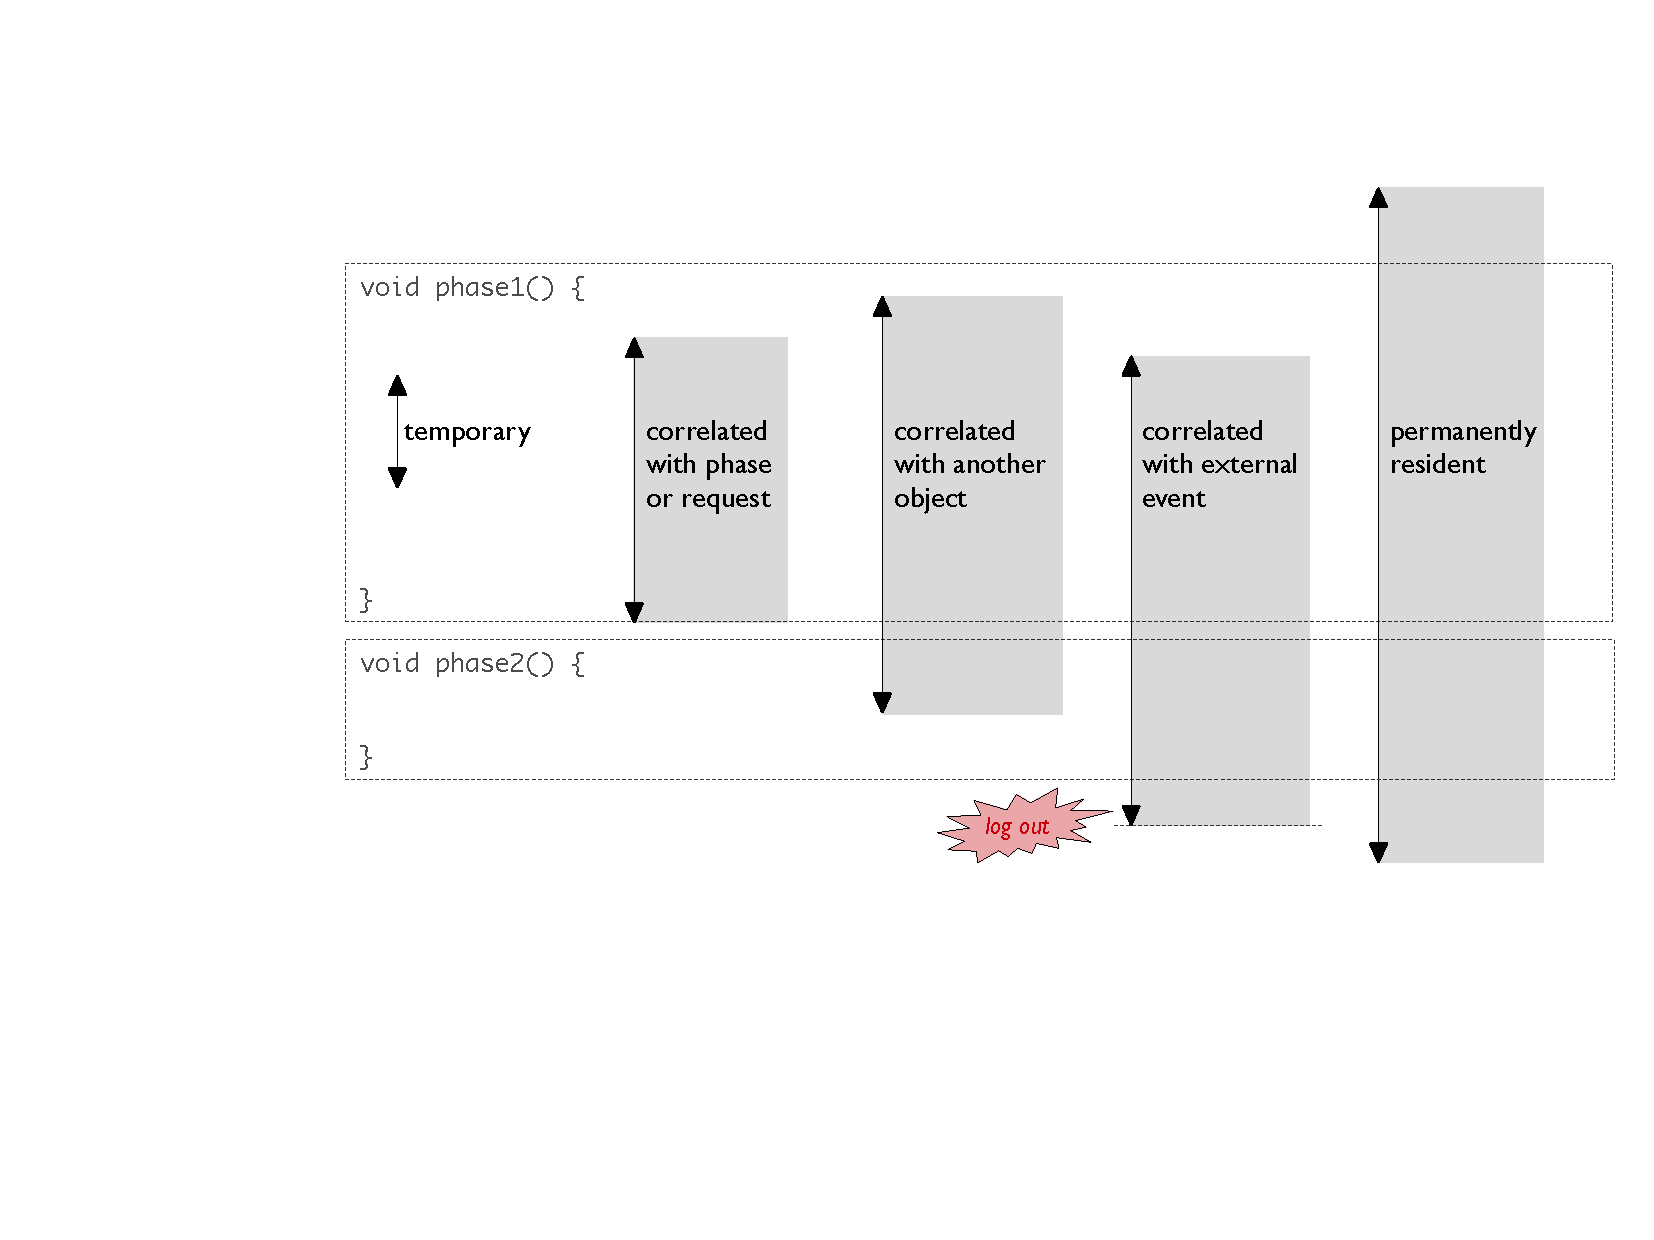
\includegraphics[width=\textwidth]{part2/Figures/lifetime/requirements}
\caption{Illustration of some common lifetime requirements.}
\label{fig:five-lifetimes}
\end{figure}

Once you have mapped out the lifetime requirements of your data models, the next
step is to chose the right implementation details in order to correctly implement
each requirement. The remaining chapters in this part show how to implement these
requirements.

%The trickier aspects of memory management, summarized in
%\autoref{tab:tricky-memory-management}, are discussed in greater detail in
%later chapters.


\section{Object Lifetimes in A Web Application Server}

%Configuring memory settings is an iterative process. It usually involves a
%fair amount of trial and error, as one tunes the various knobs to balance memory
%consumption and application performance. These knobs affect things like the size of the Java
%heap, how many entries a cache should hold, and the timeout value for these
%caches. This is usually a process of black box tuning: twist a knob, and see
%how overall performance changes. In addition to being hit
%and miss, it is also quite prone to bugs. If you set the size of a cache too
%high, you risk poor performance due to excessive garbage collection, and even
%possibly process failures, due to running out of heap space.

To introduce the common requirements for object lifetime, we walk through several
scenarios found in most long-running server applications. These applications
provide an interesting case study for lifetime management. Managing lifetime when
the application runs forever is an especially complex issue. This is true for
more than for servers alone. Desktop applications such as the Eclipse integrated
development environment shares many of the same challenges. Improperly managing
the lifetimes of objects, for short-running applications, often does not result
in critical failure. Indeed, the application often finishes its run before one
would even notice a problem with memory consumption. Plus, you're probably don't
run many instances of a short-running application simultaneously; and so
achieving the ultimate in scalability is not a primary concern. In contrast, if
an application runs more or less forever, then mistakes pile up over time. In
addition, caching plays a large role in these applications, since they often
depend on data fetched from remote servers, or from disk, neither of which can
support the necessary throughput and response time requirements. The ability for
mistakes to pile up, and for misconfigured or poorly implemented caches to impede
performance means that special care must be taken when implementing your server application.

The heap consumption of this application will fluctuate over time. A timeline
view of expected memory consumption helps to visualize these changes. It
visualizes memory during the lulls and peaks of activity, as requests are
processed and when sessions time out, and as the server starts up. We will use
these over the next few pages, as we walk through the common cases of lifetime
requirements.




% \begin{example}{Lifetime in A Web Application Server}
To help introduce the common lifetime requirements, we walk through an example of
a shopping cart server application. The server, on startup, preloads catalog data
into memory to allow for quick access to this commonly used data. It also
maintains data for users as they interact with the system, browsing and buying
products. Finally, it caches the response data that comes from a remote service
provider that charges per request. The remainder of this chapter walks you
through understanding the lifetime requirements of these data structures.
% How does Java heap consumption vary over time? Which heap size fluctuations
% indicate a problem, and which are expected behavior? \end{example}

\section{Temporaries}
\label{sec:temporary-lifetime}
\index{Temporary Objects}

The catalog data and session state are both examples of objects that are expected
to stick around for a while. In the course of preloading the cache and responding
to client requests, the server application will create a number of objects that
are only used for a very short period of time.
They help to faciliate the main
operations of the server. These temporary objects will be reclaimed by the \jres
garbage collector in relatively short order. The point at which an object is
reclaimed depends on when the garbage collector notices that it is reclaimable.
Normally, the garbage collector will wait until the heap is full, and then
inspect the heap for the objects that are still possibly in use. In this way, the
area under the \emph{temporaries} curve has a see-saw shape. As the temporaries
pile up, waiting for the next garbage collection, they contribute more and more
to memory footprint. Normally, once the \jre runs a garbage collection, these
temporaries no longer in use will no longer contribute to heap consumption.

In this way, temporary objects \emph{fill up the headroom} in the
heap.\index{Heap Headroom} If there is a large amount of heap space unused by the
longer-lived objects, then the temporaries can be reclaimed less often. This is a
good thing, because a garbage collection is an expensive proposition. \index{Heap
Size Settings} \index{Maximum Heap Size} \index{-Xmx command line setting} When
configuring your application, you may specify a maximum heap size. It should
certainly be larger than the baseline and session data. How much larger than
that? This choice directly affects the amount of \emph{headroom}, that is the
amount of space available for temporaries to pile up.

\begin{figure}
	\centering
	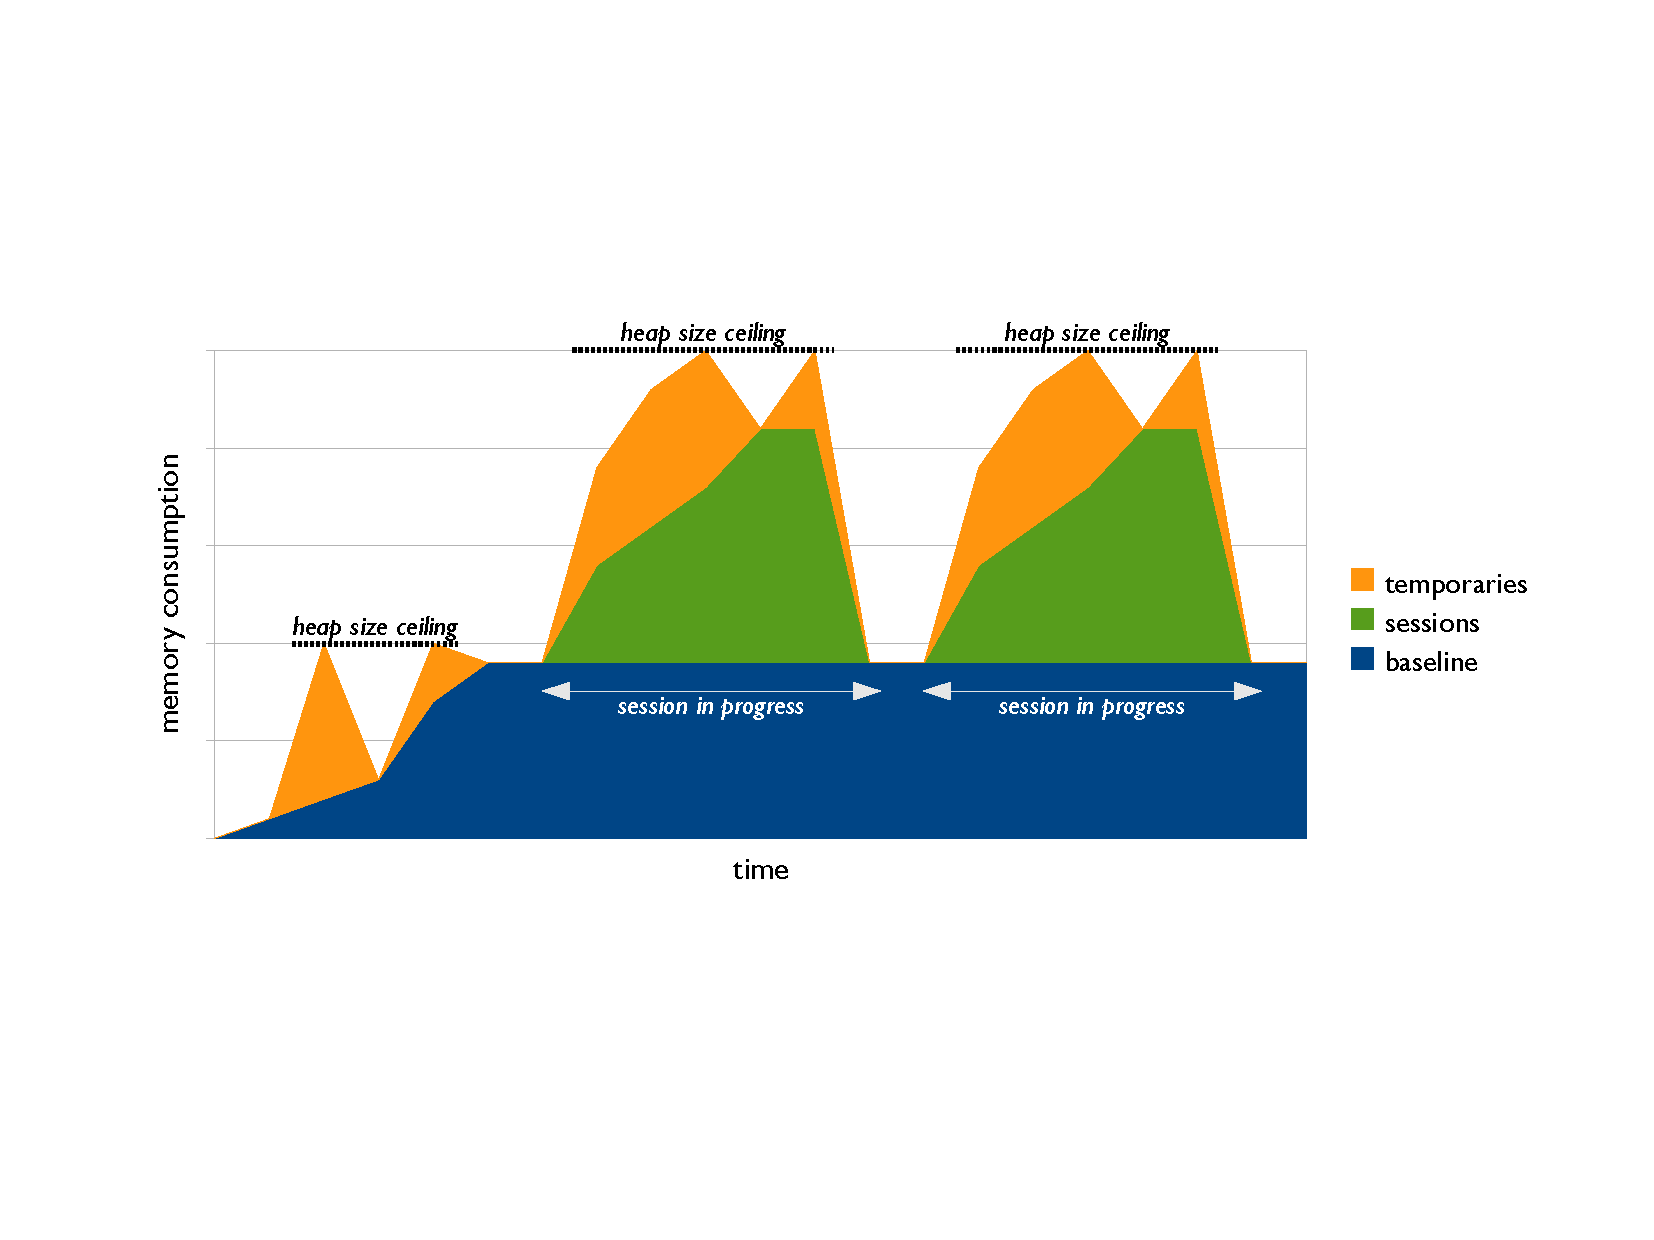
\includegraphics[width=\textwidth]{part2/Figures/lifetime/timeline-base-session-temps}
	\caption{Memory consumption, over time, typical of a web application server.}
	\label{fig:timeline-base-session-temps}
\end{figure}

\paragraph{Temporaries in Practice}
If your application is like most Java applications, it creates a large number of
these temporary objects. They hold data that will only be used for a very short
interval of time. It is often the case that the objects in these transient data
structures are only ever reachable by local variables. For example, this is the
case when you populate a \class{StringBuilder}, turn it into a \class{String},
and then ultimately (and only) print the string to a log file. The point at
which these objects, the string builder, string, and character arrays, are no
longer used is only shortly after they are constructed:

\begin{shortlisting}
String makeLogString(String message, Throwable exception) {
	StringBuilder sb = new StringBuilder();
	sb.append(message);
	sb.append(exception.getLocalizedMessage());
	return sb.toString();
}
void log(String message, Throwable exception) {
	System.err.println(makeLogString(message, exception));
}
\end{shortlisting}

A temporary object serves as a transient home for your data, as it makes its way
through the frameworks and libraries you depend on. Temporaries are often
necessary to bridge separately developed code and enable code reuse. The above
example avoids code dupliation and ensures uniformity of the output data by
factoring out the logic of formatting messages into the \code{makeLogString}
method.

%By converting your data layout into a form that an API requires,
%then you can reuse the functionality it provides.

In many cases, the \jre will do a sufficient job in managing these temporary
objects for you. Generational garbage collectors \index{Generational Garbage
Collection} these days do a very good job digesting a large volume of temporary
objects. In a generational garbage collector, the \jre places temporary objects
in a separate heap, and thus need only process the newly created objects, rather
than all objects, during its routine scan.

There are two potential problems that you may encounter with temporary objects.
The first is the runtime cost of initializing the state of the temporary
objects' fields. Even if allocating an freeing up the memory for an object is
free, there remains the work done in the constructor:

\begin{shortlisting}
class Temp {
	private final Date date;
	
	public Temp(String input) { // constructor
		this.date = DateFormat.getInstance().parse(input);
	}
}
\end{shortlisting}

Even if an instance of \class{Temp} lives for only a very short time, its
construction has a high cost. It is often the case that this expense is hidden
behind a wall of APIs. If so, then what you think of as trivial temporary (since
you, after all, are in control of when the instance of \class{Temp} lives and
dies), would in actuality be far from trivial in runtime expense. Expenses can
pile up even further if temporary object constructions are nested.

There is a second potential problem with temporary objects. By creating temporary
objects at a very high rate, it is possible to overwhelm either the garbage
collector, or the physical limitations of your hardware. For example, at some
point, the memory bandwidth necessary to initialize the temporary objects will
exceed that provided by the hardware. Say your application fills up the temporary
heap ever second. In this case, based on the common speeds of garbage collectors,
your application could easily
 spend over 20\% of its time collecting garbage. Is it difficult to fill up the
 temporary heap once per second? Typical temporary heap sizes run around 128
 megabytes. Say your application is a serves a peak of 1000 requests per second,
 and creates objects of around 50 bytes each. If it creates around 2500
 temporaries per request, then this application will spend 20\% of its time
 collecting garbage.


%A great many of these
%temporary structures serve the role of a kind of lubricant, making it easy for
%you to write code that ties together the separately written parts of your code
%base and reuses standard libraries as much as possible. Often, these are
%objects that are not a fundamental necessity of what you're trying to
%accomplish. If
%you had the freedom to code highly specialized implementations of the important
%cases, from scratch, many of these temporary structures would be unnecessary.

\begin{example}{How Easy it is to Create Lots of Temporary Objects}
A common example of temporaries is parsing
and manipulating data coming from the outside world. Identify the temporary
objects in the following code.
% to the wire?

\begin{shortlisting}%[float,caption=Code that constructs 8 temporary objects tohandle two dates.,label=TempExampleCode]
void main(String xy) {
	doWork(xy.substring(0,10), xy.substring(10));
}	
void doWork(String x, String y) {
	doRemoteProcedureCall(parse(x));
	doRemoteProcedureCall(parse(y));
}
Date parse(String string) {
	return DataFormat.getInstance().parse(string, new ParsePosition(0));
}
void doRemoteProcedureCall(Date date) {
	long timestamp = date.getTime();
	...
}
\end{shortlisting}
\end{example} 

This code starts in the \code{main} method by splitting the input string into two
substrings. So far, the code has created four objects (one \class{String} and one
character array per substring). Creating these substrings makes it easy to use
the \code{doWork} method, which takes two Strings as input. However, observe that
these four objects are not a necessary part of the computation. Indeed, these
substrings are eventually used only as input to the \class{DateFormat}
\code{parse} method, which has been nicely designed to allow you to avoid this
very problem. By passing a \class{ParsePosition}, one can parse substrings of a
string without having to create temporary strings (at the expense of creating
temporary \class{ParsePosition} objects).



\section{Time-space Tradeoffs}
\label{sec:time-space-tradeoffs-pattern}
\index{Time-Space Tradeoffs}

\begin{figure}[h]  % NMM added [h] just to make formatting look good on 201007014, not necessary
	\centering
	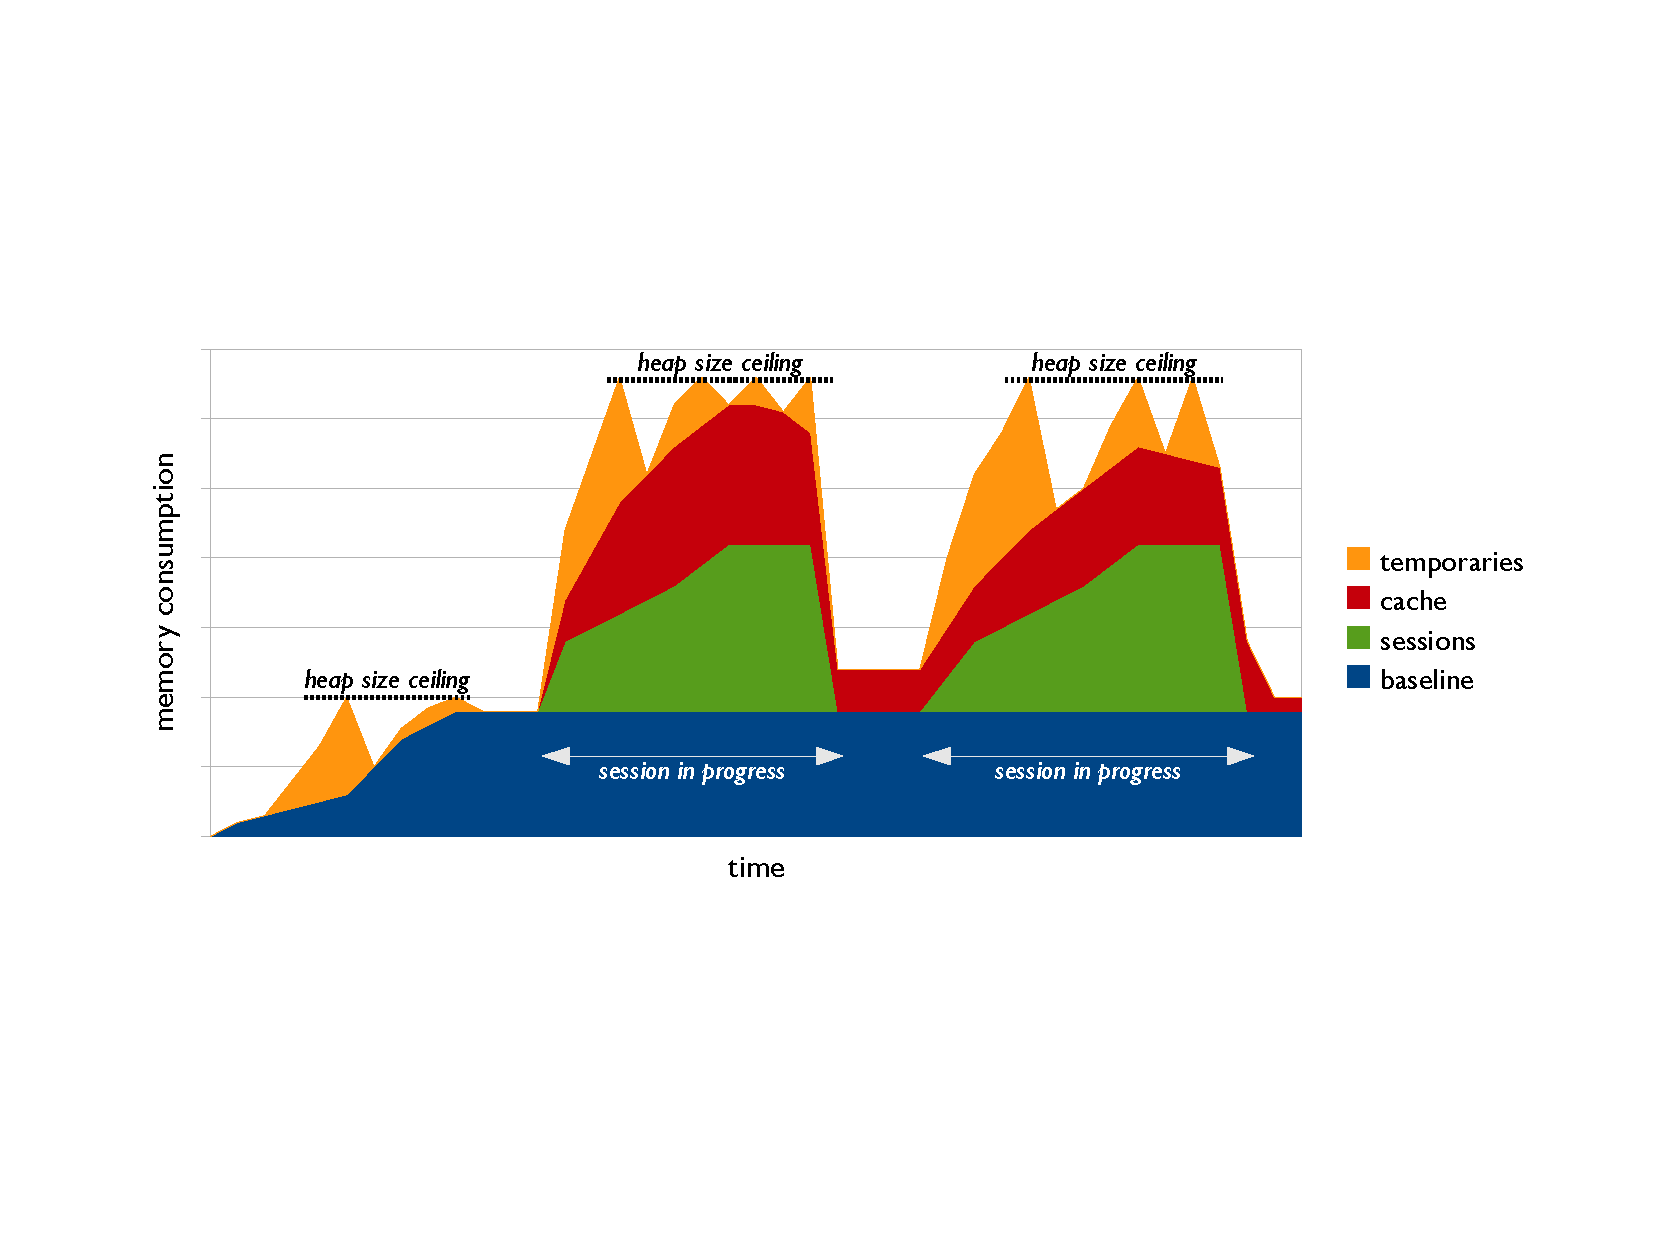
\includegraphics[width=\textwidth]{part2/Figures/lifetime/timeline-base-session-temps-with-cache}
	\caption{When a cache is in use, this leaves less headroom for temporary
	object allocation, often resulting in more frequent garbage collections.}
	\label{fig:timeline-base-session-temps-with-cache}
\end{figure}

Sometimes it is beneficial to extend, or shorten, the lifetime of an object. For
example, if every request creates an object of the same type, with the same, or
very similar, fields, then you should consider caching or pooling a single
instance of this object. There are four important cases of time-space tradeoffs.
The first covers the situation where recomputing attributes, rather than storing
them, is a better choice. The next three cover situations where spending memory
to extend the lifetime of certain objects saves sufficient time to be worthwhile:
caches, sharing pools, and resource pools.
\autoref{chapter:lifetime-implementation-strategies} discusses implementation
strategies for these situations.

The example server caches data from an expensive third-party data source. Caching
external data in the Java heap complicates your programming and management tasks.
The cache must be configured properly so that its contents live long enough to be
amortize their costs of fetching, while not occupying too much of the heap. If
caches are sized too large, this would leave little space for the temporaries
that your application creates.
\autoref{fig:timeline-base-session-temps-with-cache} shows an example where the
cache has probably been configured to occupy too much heap space. Observe how,
compared to the other timeline figures, there is little headroom for temporary
objects. The result is more frequent garbage collections. If the cache were sized
to occupy an even greater amount of heap space, it is possible that there would
no longer be room to fit session data. The result in this case would be failures
in client requests.

Sizing caches is important, but tricky to get right. If the data to be cached is
stored on a local disk, then another strategy to caching is to use \emph{memory
mapping}. \autoref{sec:memory-mapping} describes how to utilize built-in Java
functionality that lets you take advantage of the underlying operating system's
demand paging functionality to take care of caching for you.

\section{Correlated Lifetimes}
\label{sec:correlated-lifetime-pattern}

The catalog data should last forever, while the
session data lives for some bounded period of time. It is possible that session
state will live beyond the end of your session, but nonetheless it has a
lifetime that is bounded. If, due to an bug, part of this session state is not
reclaimed, the application will leak memory. Though it is supposed to have a bounded lifetime, it
\marginpar{\textbf{Memory Leaks} are still possible, even with
automatic garbage collection!} 
accidentally lives forever. In this
case, over time, the amount of heap required for the application to run will increase without bound.
\index{Memory Leaks}
\autoref{fig:timeline-base-session-temps-with-leak} illustrates this situation,
in the extreme case when all of session state leaks. Over time, the area under
the curve steps higher and higher.

\begin{figure}[h]  % NMM added [h] just to make formatting look good on 201007014, not necessary
	\centering
	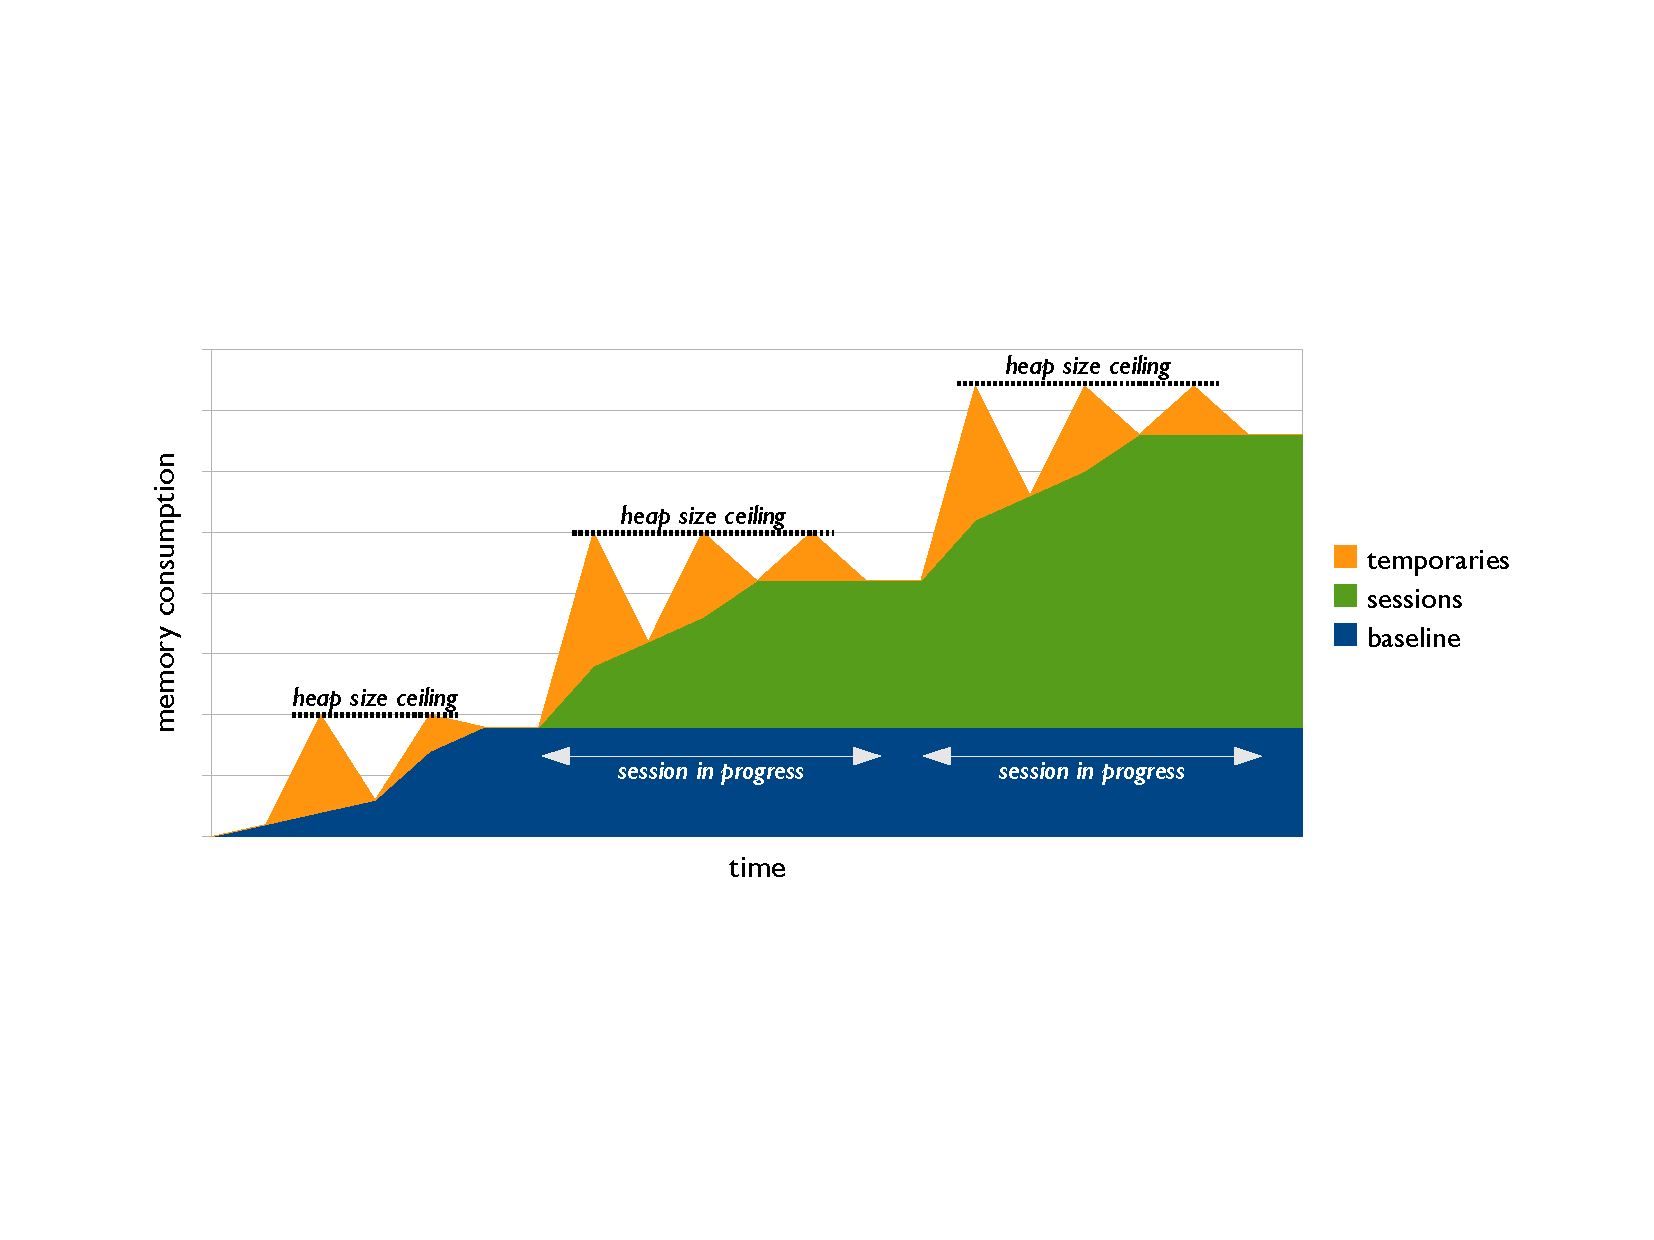
\includegraphics[width=\textwidth]{part2/Figures/lifetime/timeline-base-session-temps-with-leak}
	\caption{If session state is not cleaned up
	properly, a memory leak is the result. This means more frequent garbage
	collections, and ever increasing heap size.}
	\label{fig:timeline-base-session-temps-with-leak}
\end{figure}

%As you scan the timeline from left to right, memory consumption 
%it fetches catalog data from its database, and stores them in the Java heap. 

\paragraph{Correlated Lifetime in Practice}

Many objects are needed for a bounded interval of time. In some cases, this
interval is bounded by the lifetime of another object. In a second important
scenario, the lifetime of an object is bounded by the duration of a method call.
Once that other object is not needed, or once that method returns, then these
\emph{correlated} objects are also no longer needed. These are the two important
cases of objects with correlated lifetime.

\paragraph{Objects that Live and Die Together}
\label{sec:correlated-lifetime-1}

If you needed to augment the state stored in instances of a class that you are
responsible for, you would modify the source code of that class. For example, to
add a secondary mailing address to a \class{Person} model, you add a field to
that class and update the initialization and marshalling logic accordingly. This
works fine for classes that you own, and when most \class{Person} instances have
a secondary mailing address. Sometimes, you will find it necessary to associate
information with an object that is, for one reason or the other, locked down, or
where the attributes are only sparsely associated with the related objects.

\begin{example}{Annotations}
In order to debug a performance problem, you need to associate a timestamp with
another object. Unfortunately, you don't have access to the source code for
that object's class. Where do you keep the new information, and how can you
link the associated storage to the main objects without introducing memory
leaks?\index{Memory Leaks}
\end{example}

If you can't modify the class definition for that object, then you will have to
store the extra information elsewhere. These \emph{side annotations}\index{Side
Annotations} will be objects themselves, and you need to make sure that their
lifetimes are correlated with the main objects. When one dies, the other
should, too.

\paragraph{Objects that Live and Die with Program Phases}
\label{sec:correlated-lifetime-2}

Similar to the way the lifetime of an object can be correlated with another
object, lifetimes are often correlated with method invocations. When a method
returns, objects correlated with it should go away. For temporary objects, this
is usually easy to ensure, since they are usually only reachable from stack
locations. For the medium-to-long running methods that implement the
core functionalities of the program, this correlation is harder to get right.

For example, if your application loads a log file from disk,
parses it, and then displays the results to the user, it has roughly three
phases for this activity. Most of the objects allocated in one phase are scoped to that
phase; they are needed to implement the logic of that phase, but not subsequent
phases. The phase that loads the log file is likely to maintain maps that
help to cross reference different parts of the log file. These are necessary
to facilitate parsing, but, once the log file has been loaded, these maps can be
discarded. In this way, these maps live and die with the first phase of this
example program. If they don't, because the machinery you have set up to
govern their lifetimes has bugs, then your application has a memory
leak\index{Memory Leaks}.

This lifetime scenario is also common if your application is an
server that handles web requests.

\begin{example}{Memory Leaks in an Application Server}
	A web application server handles servlet requests. How is it possible that
	objects allocated in one request would unintentionally survive beyond the end
	of the request?
\end{example} 
  
In server applications, most
objects created within the scope of a request should not survive the
request. Most of these \emph{request-scoped}
\index{Request-scoped Lifetime} objects are not used by the application after the
request has completed. In the absence of application or framework bugs, they will
be collected as soon as is convenient for the runtime. In this example, the
lifetime of objects during a request are \emph{correlated} with a method
invocation: when the servlet \class{doGet} or \class{doPut} (etc.) invocations
return, those correlated objects had better be garbage collectible.

\index{Memory Leaks: Why?}
There are many program bugs and configuration missteps that can lead to
problems. The general problem is that a reference to an object stays around
indefinitely, but becomes
\emph{forgotten}, and hence rendered unfindable by the normal application
logic. If this request-scoped data structure were only reachable from stack
locations, you would be fine. Therefore, a request-scoped object will leak only
when there exist references from some data structure that lives forever. Here
are some common ways that this happens.

\begin{itemize}
  \item Registrars, where objects are registered as listeners to some service,
  but not deregistered at the end of a request.
  \item Doubly-indexed registrars. Here the outer map provides a key to index
  into the inner map. A leak occurs when the outer key is mistakenly
  overwritten mid-request. This can happen if the namespace of keys isn't
  canonical and two development groups use keys that collide. It can also
  happen if there is a mistaken notion, between two development groups, of who
  owns respnsibility of populating this registrar.
  \item Misimplemented hashcode or equals, which foils the retrieval of an
  object from a hash-based collection. If developers checked the return value of
  the \code{remove} method, which for the standard collections would indicate a failure to remove, then
  this bug could be easily detected early; but developers tend not to do this.
\end{itemize}

The next chapter goes into greater detail on how to avoid these kinds of
errors. \autoref{chapter:tools} describes tooling that can help you
detect and fix the bugs that make it into your finished application.


\section{Correlated with External Event}
\index{Lifetime Requirement, Correlated with External Event}
\label{sec:correlated-with-need}

After the server is warmed up, it begins to process client requests. Imagine
interacting with a commerce site with a web browser. First you browse around,
looking for items that you like, and add them to your shopping cart. Eventually,
you may authenticate and complete a purchase. As you browse and buy, the server
maintains some state, to remember aspects of what you have done so far. For
example, the server stores the incremental state of multi-step transactions,
those that span multiple page views. This session state, at least the part of it
stored in the Java heap, will go away soon after your browsing session is
complete. In the timeline figure, this portion of memory is labeled
\emph{sessions}. It ramps up while a session is in progress, and then, in the
example illustrated here, soon all of that session memory should be reclaimed.

These session state objects need to be kept around for operations that span
several independent operations, and are possibly used across multiple threads.
They are used beyond the scope of a phase, are not correlated with another
object, but don't live forever.

\section{Permanently Resident}
\label{sec:forever-lifetime}
\index{Permanently Resident Objects}

\autoref{fig:timeline-base-session-temps} shows the timeline of memory
consumption of our example server 
during and shortly after its initial startup.
During the startup interval, the server preloads catalog data into
the Java heap. Then, the server is warmed with with two test requests.
The total height of the area
under the curves represents the memory consumption at that point in time. 
The preloaded catalog
data will be used for the entire duration of the server process.
\index{Objects That Live Forever}
Therefore, the Java objects that represent this catalog are objects that are
needed forever. In the timeline picture, this data is respresented by the lowest area, labeled
\emph{baseline}. Notice how it ramps up quickly, and then, after the server has
reached a ``warmed up'' state, memory consumption of this baseline data evens out
on a plateau for the remainder of the run.

\paragraph{Permanently Resident Objects in Practice}

In the above example, a \class{DateFormat} object was created in every loop
iteration and used only once. We can improve this situation by creating and using
a single formatter for the duration of the run. The Java API documentation, in
writing at least, encourages this behavior, but leaves the burden of doing so on
you. You must be careful to remember that it is not safe to do so in multiple
threads. The next chapter will discuss remedies to this problem. The updated code
for the \code{parse} method would be:

\begin{shortlisting}
static final DateFormat fmt = new DateFormat.getInstance();

Date parse(String string) {
	return fmt.parse(string, new ParsePosition(0));
}
\end{shortlisting} 

There are other cases where your application routinely accesses data structures
for the duration of the program's run. For example, if your application loads in
trace information from a file and visualizes it, then the data models for the
trace data cannot be optimized away entirely. Sometimes it is possible, but not
practical from a performance perspective, to reload this data. You could
architect your program so that subsets of the trace data are re-parsed as they
are needed. Unfortunately, the resulting performance, or the complexity of the
code, may suffer drastically. If so, these data structures must, for practical
purposes, reside permanently in the heap.

\paragraph{When Objects Don't Fit}
Sometimes, despite your best efforts at tuning these long-lived data structures,
the structures still don't fit within your given Java heap constraints.
\autoref{chapter:large-long-lived} discusses strategies for coping with this
situation.

% introduced by example in this chapter, and
%Many objects are either temporaries or needed for
%the entire run of your application. Sometimes you create objects whose lifetime
%is correlated with other objects or that should go away when a method
%invocation completes. Sometimes you need to manage objects hanging around
%longer than their current need, to avoid future recomputations or refetching
%of data in the case when it is needed in the near future. 

%\begin{table}
%\centering
	%\begin{tabular}{ll} \toprule
    %%%%	%& Things Java Doesn't Do Automatically \\ \cmidrule{2-2}
%    	\autoref{avoiding-lifetime-bugs} & {Avoiding Memory Leaks} \\
%    	\autoref{balance-time-and-space} & {Balancing Time and Space} \\
%    	\autoref{outisde-java-box} & {Supporting Massive Data Sets}  	\\
%        \bottomrule
%    \end{tabular}
%	\caption{The tricky aspects of memory management.}
%	\label{tab:tricky-memory-management}
%\end{table}




% correlated with need: as soon as last user goes away, remove his stuff 
% share common expressions to save space, but using strong references -> memory
% leak; plugins in eclipse go away when all views
% sharing pool 

% weak ref keys -> annotation
% weak ref values -> sharing pool

% soft ref values -> caching

% annotation by map lookup










%% OLD STUFF NMM 20090820
%\section{Request Scoping}
%\section{Correlated Lifetime}
%\paragraph{Weak and Soft references in Java}
%\section{Memory Leaks and Drag}
%\section{Examples}
%\subsection{Transient Near-Copies}
%\subsubsection{String Canonicalization}
%\subsection{Temporary Collections}
%\subsection{Facilitators}

% TODO maybe introduce weaks and softs??

\chapter{Memory Management Fundamentals}

% Before getting into the details of how to implement your lifetime
% requirements,
The Java language has a \emph{managed runtime}. In part, this means that, as a
Java program runs, the Java runtime takes on the burden of key aspects of memory
allocation and reclamation. It is important to understand what Java does for
you, in forming its decision of when an object should be reclaimed, when
devising your lifetime management strategy. This level of management includes
automatic garbage collection of both instances and Java classes. Java has
feature that govern, on your behalf, important aspects of the lifetime of
objects. Unfortunately, these features often appear in the form of low-level JVM
hooks, or implicit behavior that you have to carefully govern, and so require
careful coding to make correct use of them. You need to appreciate what the
runtime is doing for you, before considering how to reshape object lifetimes to
better suit your needs.

\section{Managed Memory}

When you write Java code that allocates objects, the \jre a

\paragraph{Heaps and Stacks}


\begin{figure}
\centering
	\subfigure[When
	using
	Java,
	the stack can
	contain only primitive data and pointers to heap objects; each of those heap
	objects has a header that the \jre tacks on, for its own management
	purposes.]{\label{fig:heaps_and_stacks_java}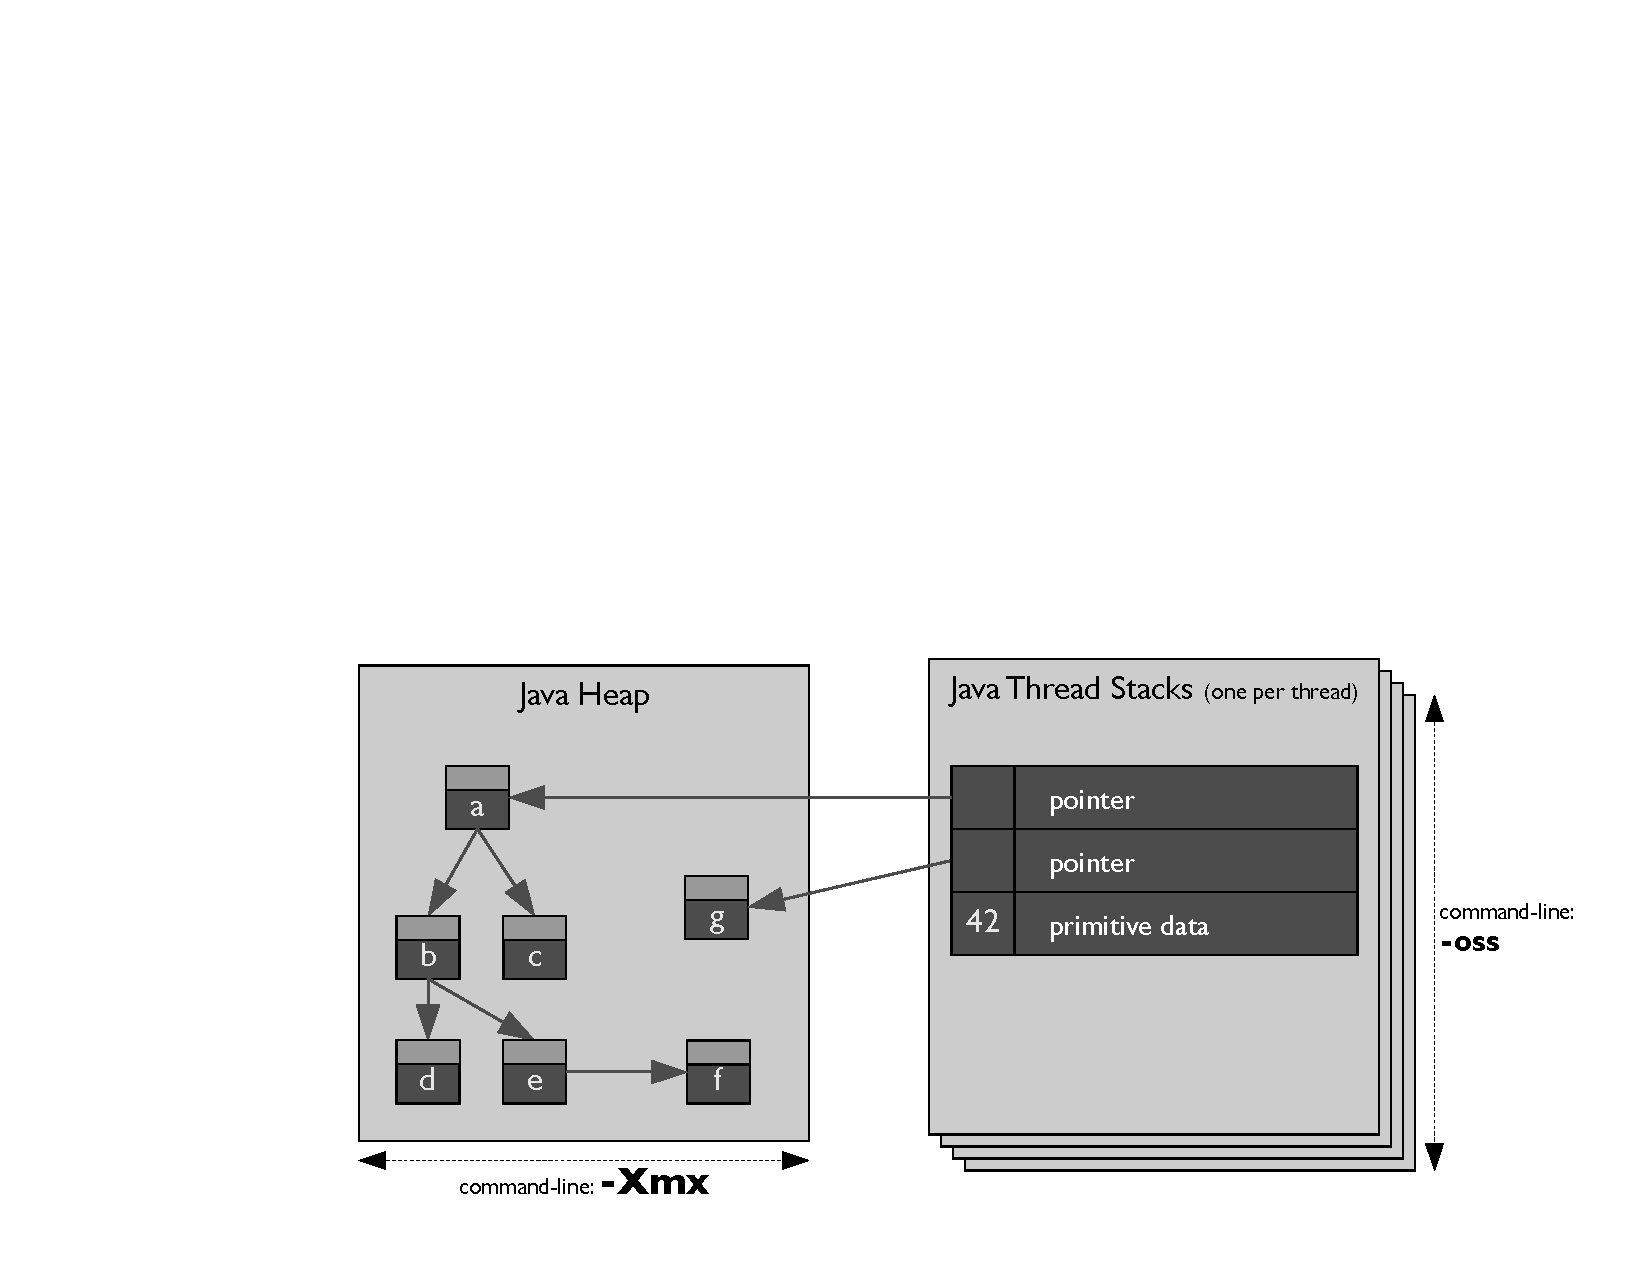
\includegraphics[width=0.75\textwidth]{part2/Figures/lifetime/heaps_and_stacks_java}}
	%\qquad
	\subfigure[When
	using
	native code, such as when coding in C,
	the stack can also contain allocated storage ({\tt
	structs}), and allocated storage can include
	other structures that have been inlined ({\tt d} has been inlined into {\tt
	b}); there are no headers in C, since it is not a managed language.
	]{\label{fig:heaps_and_stacks_C}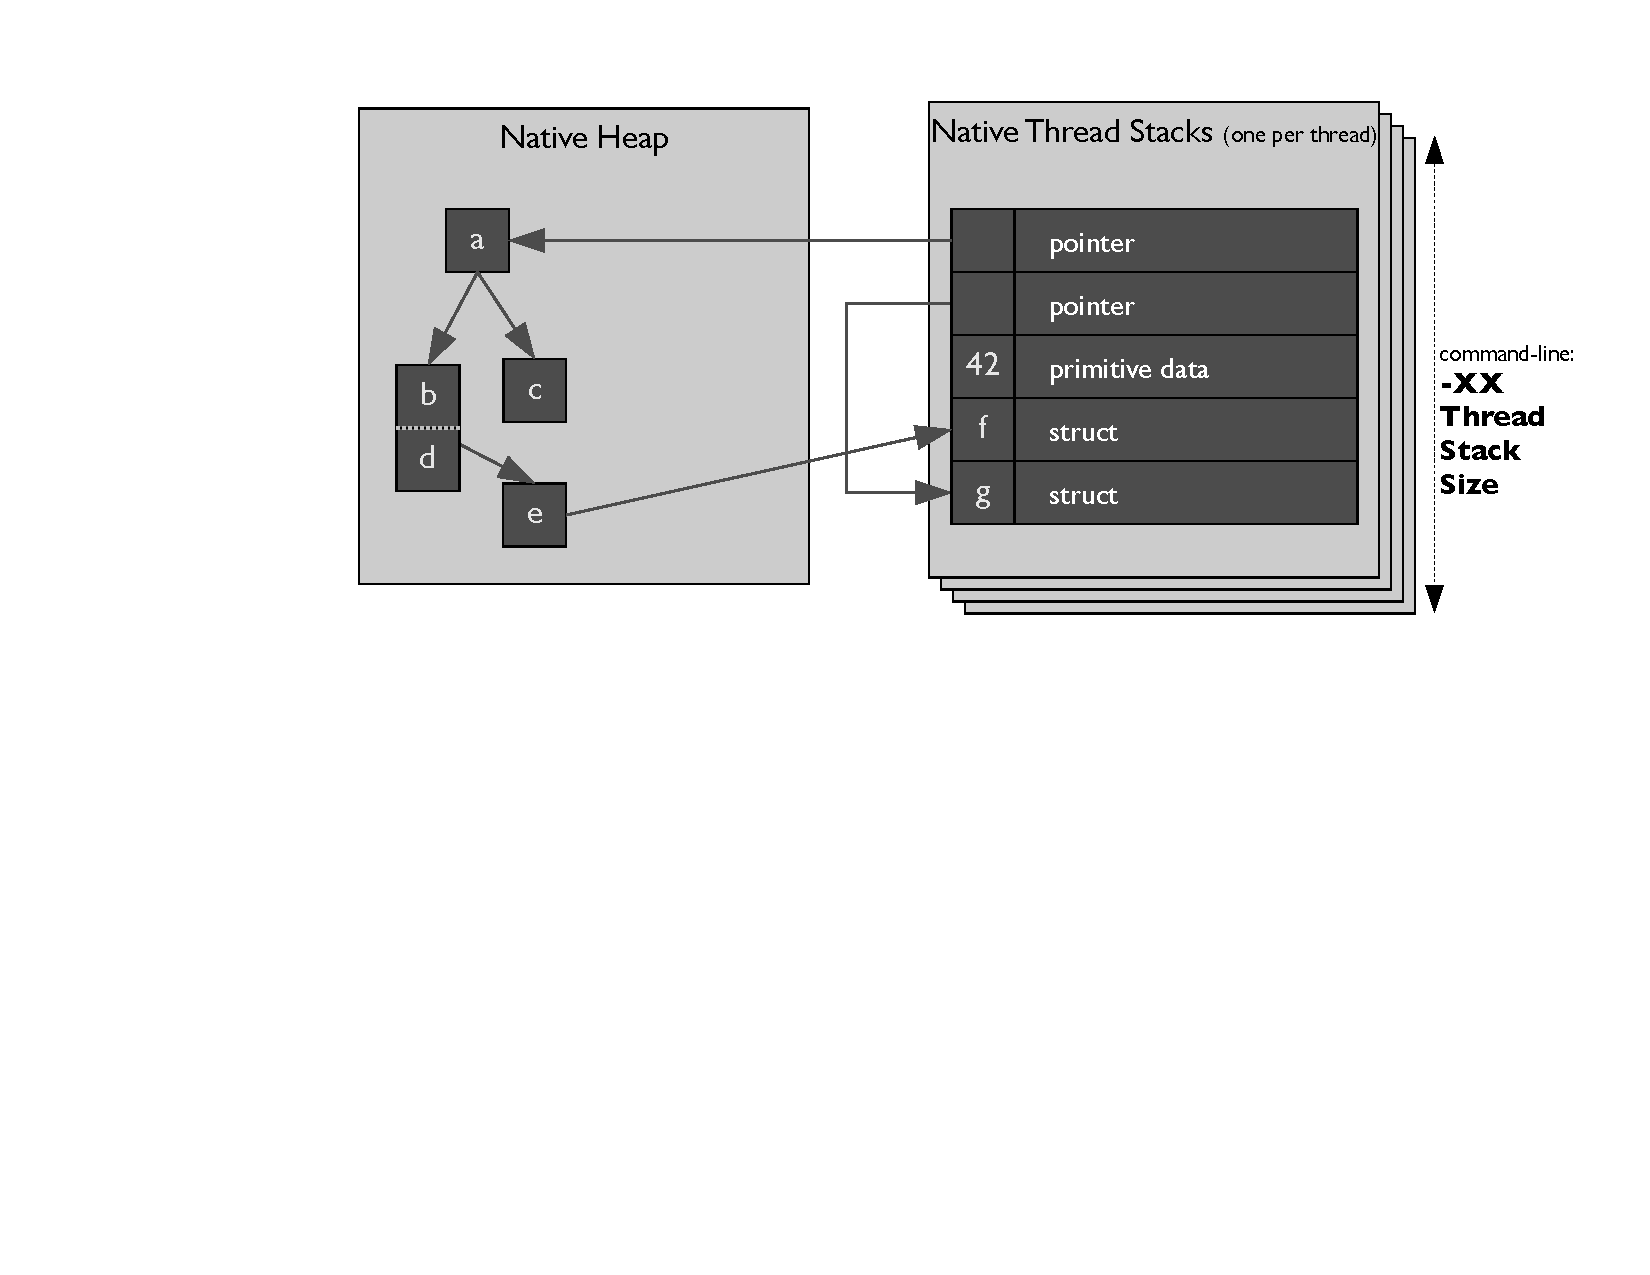
\includegraphics[width=0.75\textwidth]{part2/Figures/lifetime/heaps_and_stacks_C}}
	\caption{Your data is stored on the heap and the stack. } \subfigure[The \jre also manages classes and compiled code, but in separate
	heaps. With some \jres, this data is combined into a single heap, called the
	\emph{Permspace}
	heap,
	which
	is
	sized
	via
	{\tt
	-XX:MaxPermSize}.]{\label{fig:heaps_and_stacks_C}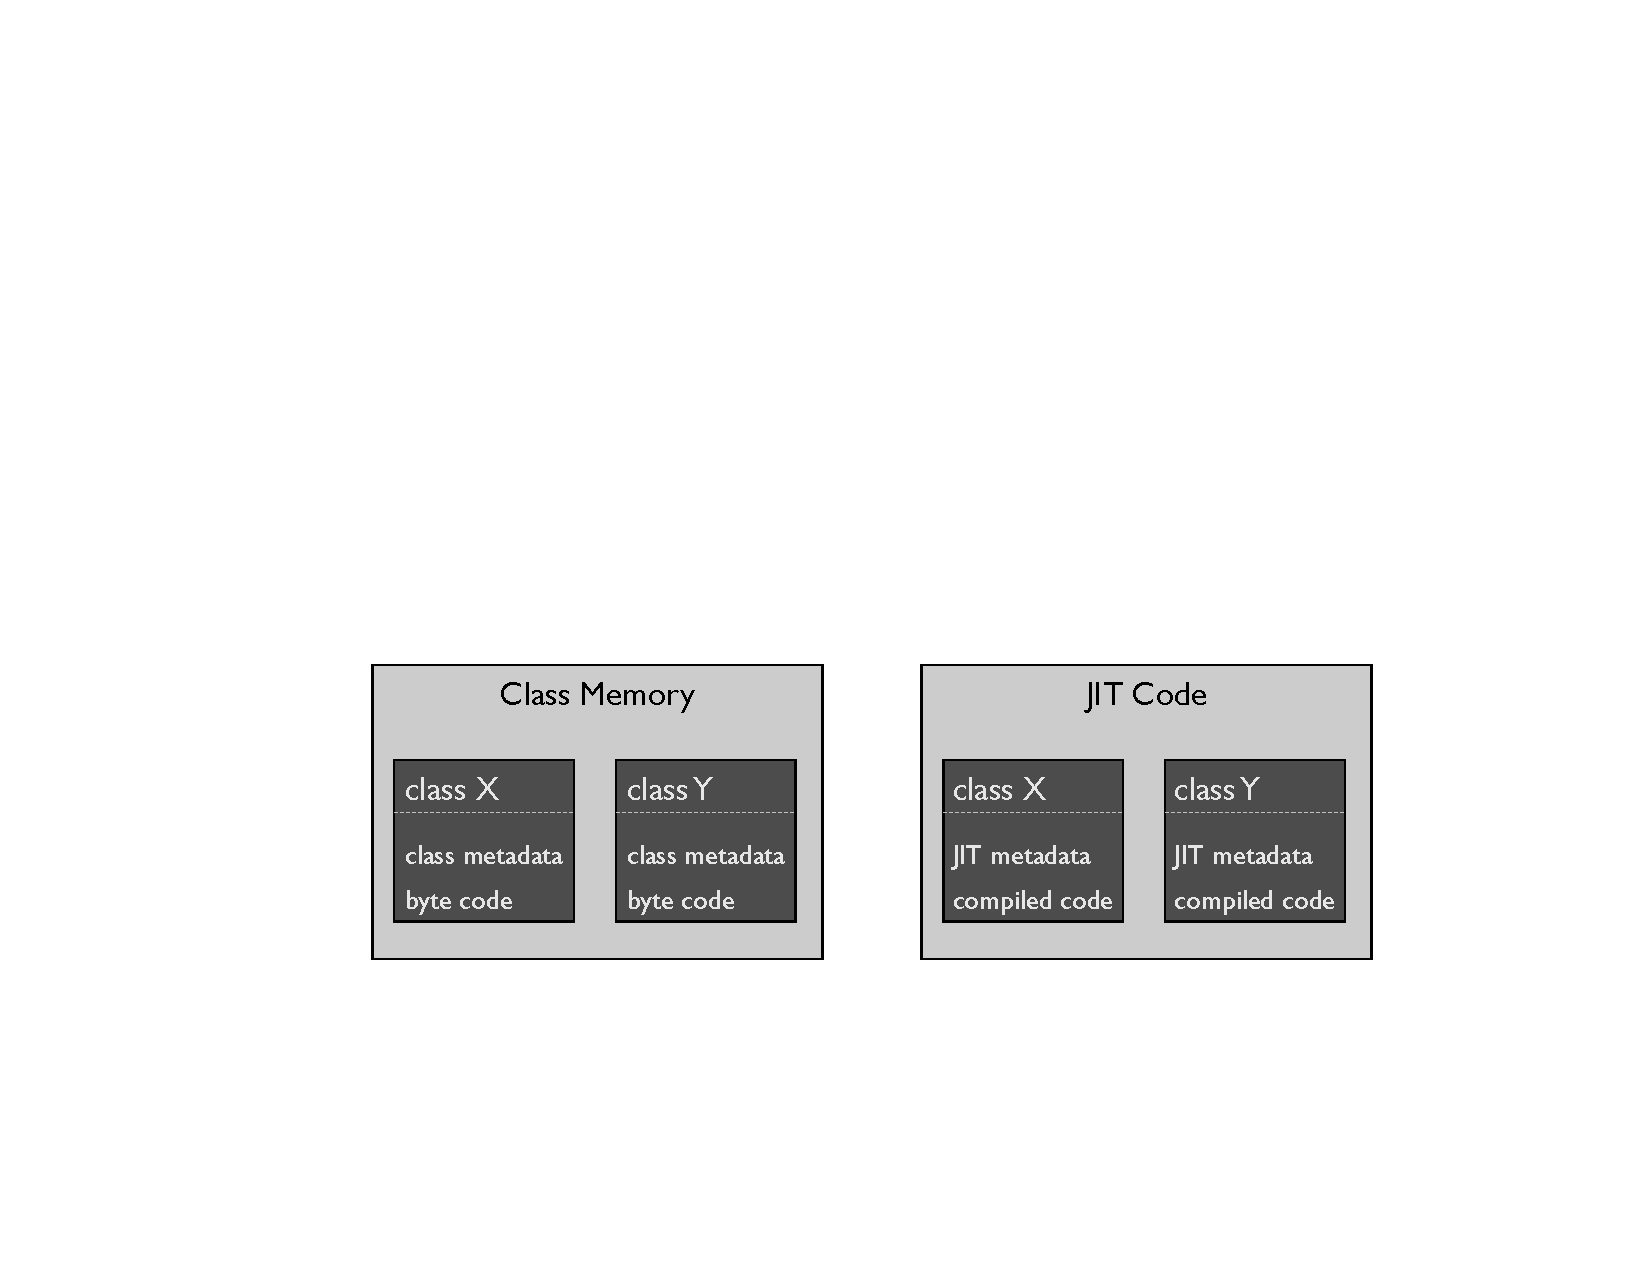
\includegraphics[width=0.75\textwidth]{part2/Figures/lifetime/heaps_and_stacks_classes}}
	\caption{Your data is stored on the stack and various heaps. }
	\label{fig:heaps_and_stacks}
\end{figure}

\paragraph{The Java vs. Native Heap}


\paragraph{Managed Objects}


%Designing a lifetime management strategy requires that you take the tools that
%Java provides, and combine them with other strategies implemented on top of
%Java. The built-in mechanisms handle some aspects of the common patterns of
%object lifetime. 

%This chapter introduces the basics of the garbage collector, and how the Java
%managed runtime governs object lifetimes. Then, it walks you through the
%lifecycle of typical objects from allocation to eventual garbage collection. If
%you are comfortable with the basics of memory management, you may discover that
%you can skip to the next chapter.

\paragraph{The Garbage Collector}
The garbage collector is the mechanism for determining when an object should be
reclaimed. It is governed by a number of configuration choices that you can make.
These configuration choices guide the schedule that the collector follows. This
includes, for example, the frequency of collection and the lengths of pauses your
application experiences. In any case, the collector will obey some basic
principles, dictated by how your data structures are interconnected, when
determining \emph{what} to collect.

%\paragraph{What a Collection Collects: Reachability and Unique Ownership}
Each time a garbage collection occurs, the collector inspects the heap for
possibly \emph{live} objects. The collector treats the heap as a graph of
objects. The nodes are the objects themselves, and the edges are field or array
slots that result in a pointer from one object to another. \index{Heap, as a
graph of objects} Recursively, an object is live either if it is a referenced
either by a live object, or, in the base case, by a \emph{root}. The roots of
garbage collection are those that come from outside the Java space, and include:
objects serving as monitors, objects on the stack of a method invocation in
progress, and references from native code via the Java Native Interface (JNI).
Every other object not live, in this sense, are ready for collection; they are
garbage.

\begin{figure}
\centering
	\subfigure[A live data
	structure.]{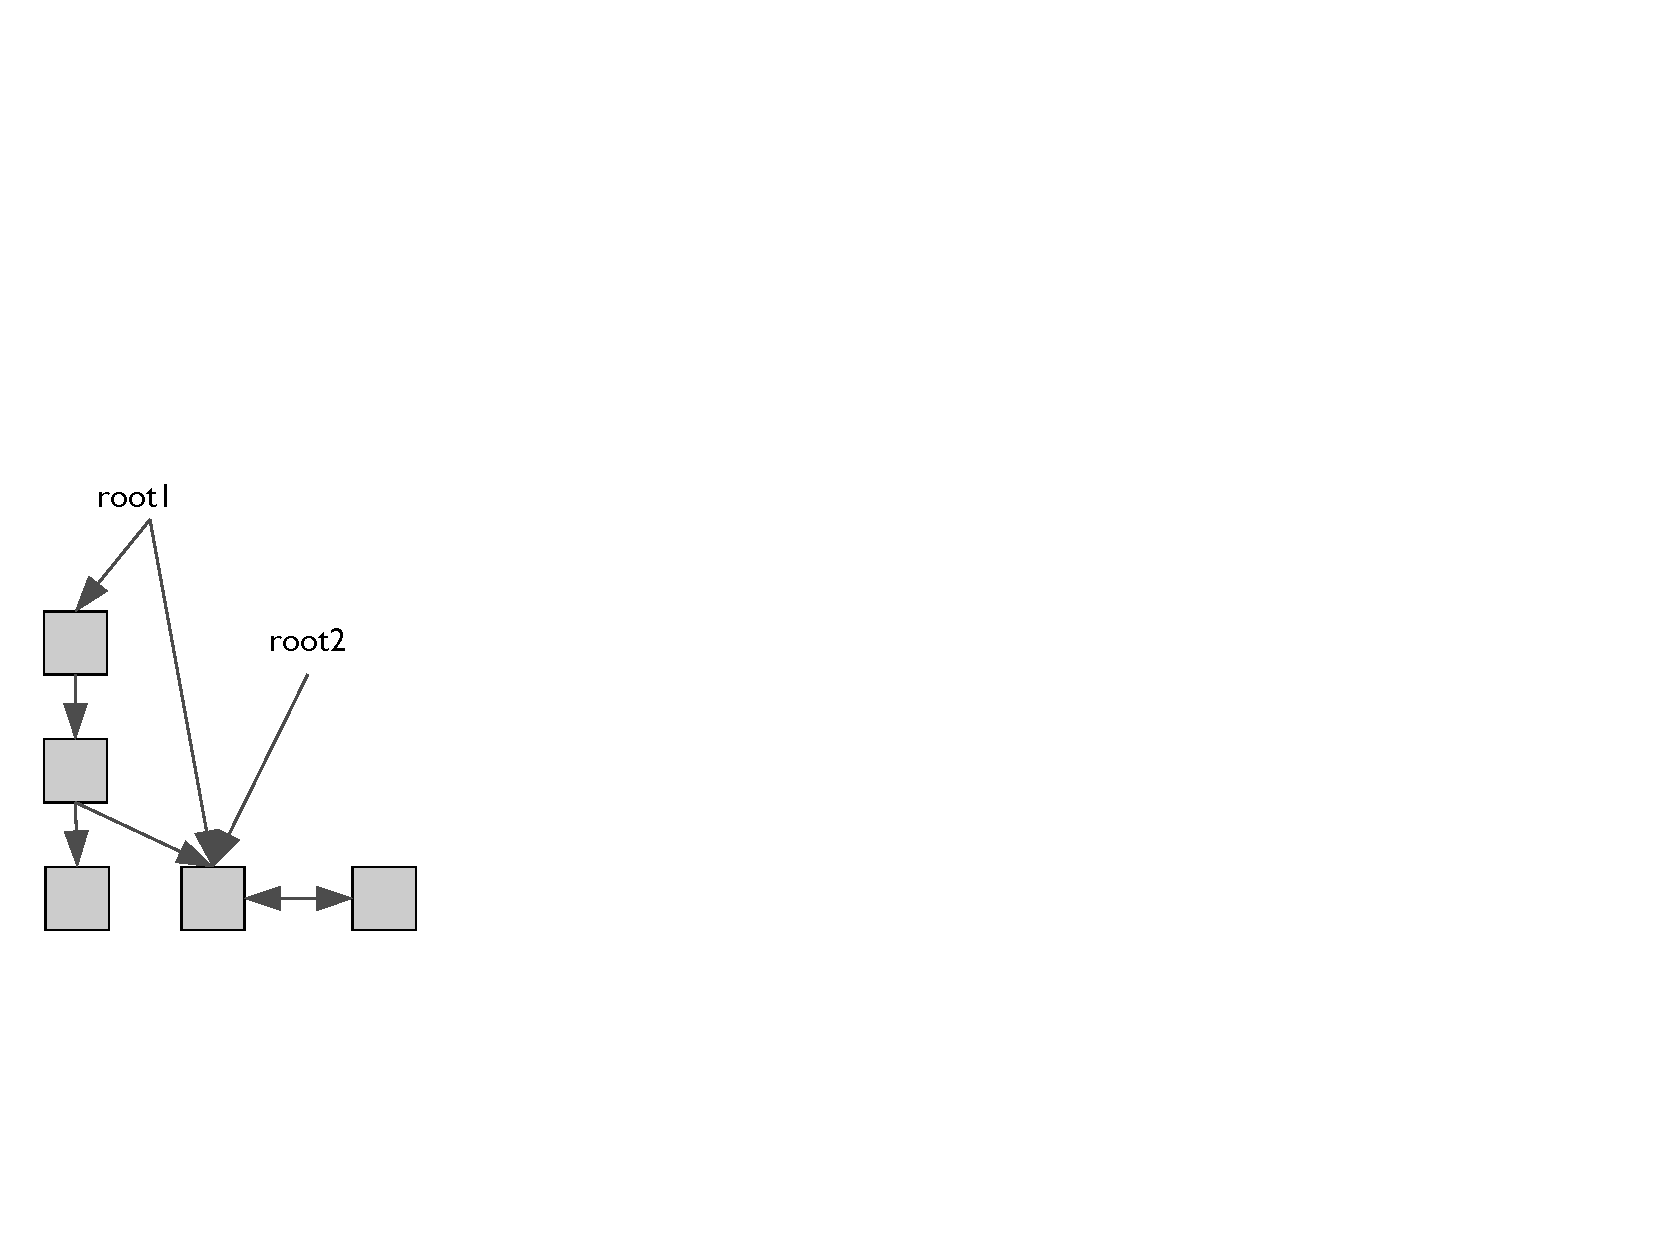
\includegraphics[width=0.3\textwidth]{part2/Figures/lifetime/reachability1}}
	\hspace{0.18\textwidth}
	\subfigure[Then, the dominating reference is
	clipped.]{\label{fig:reachability-b}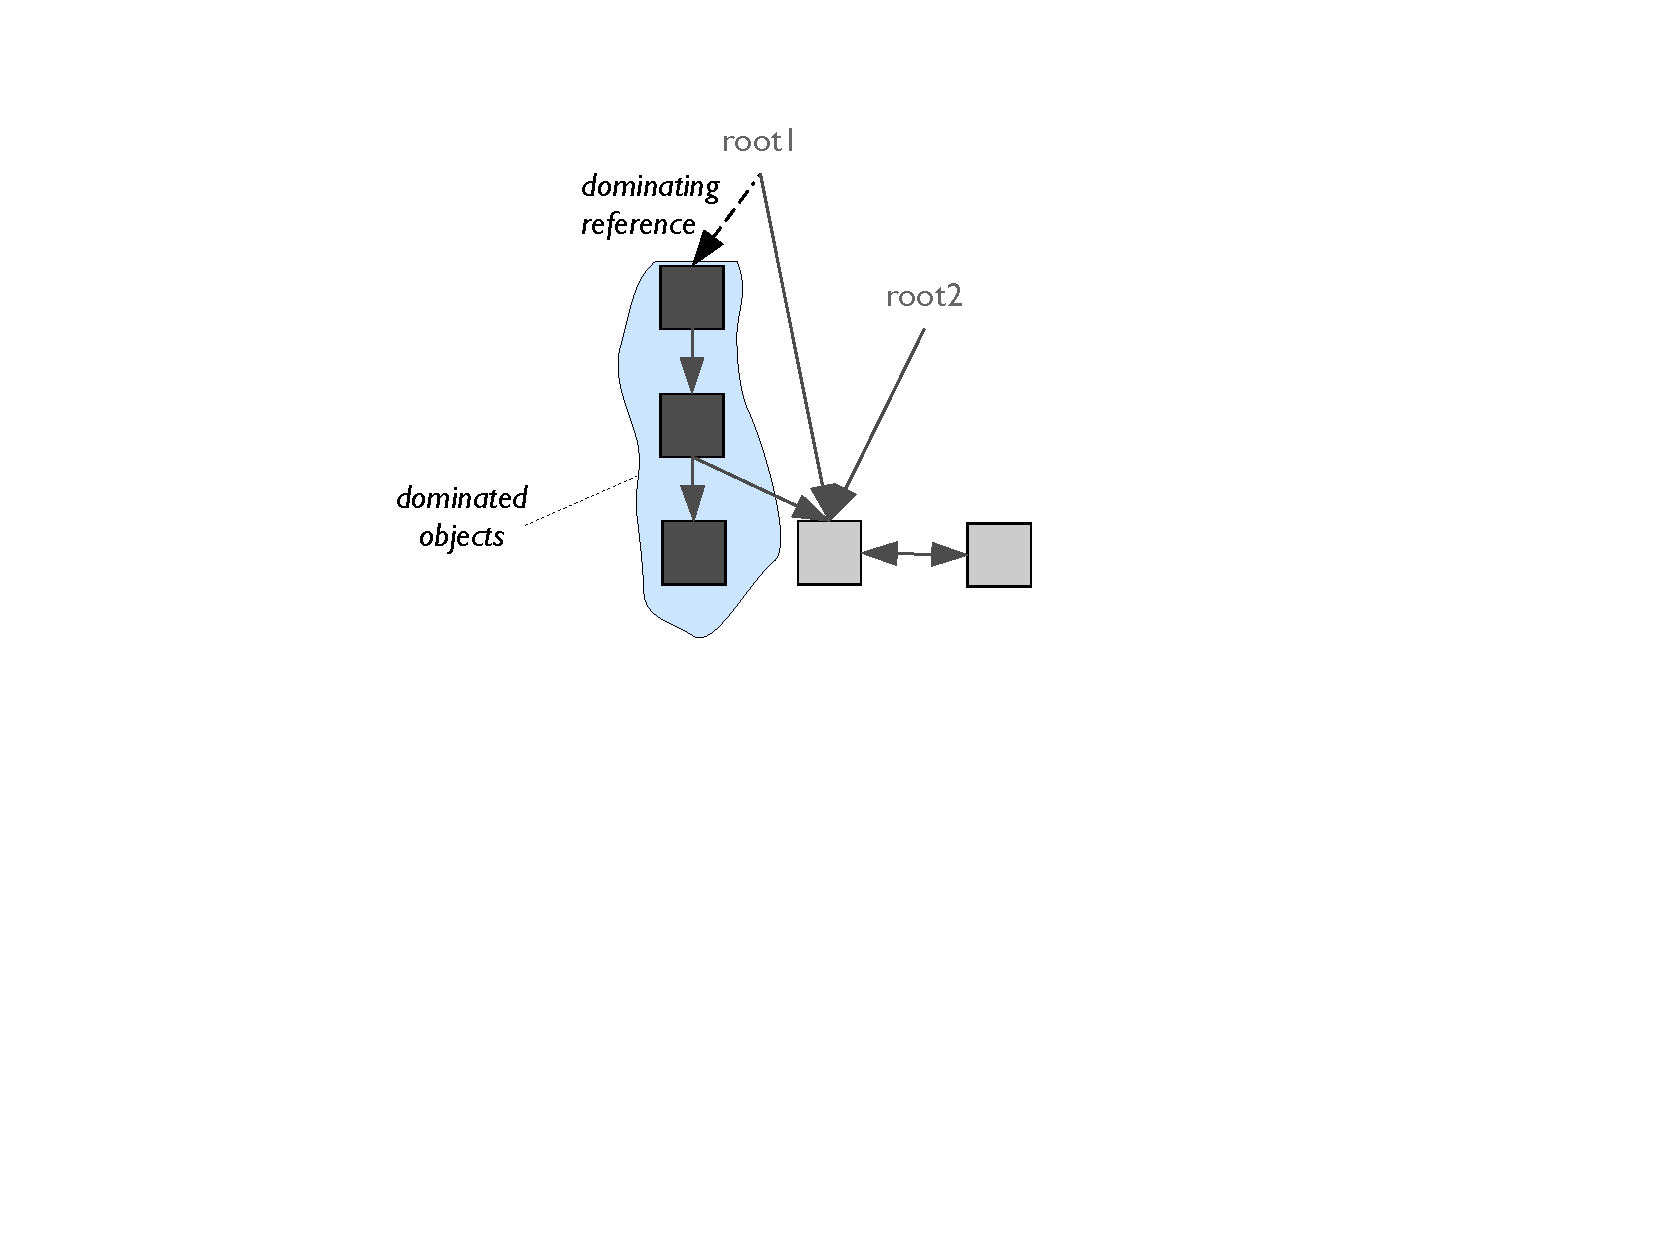
\includegraphics[width=0.445\textwidth]{part2/Figures/lifetime/reachability2}}
	\caption{The garbage collector uses the references between objects to
	determine what objects are collectable. The data structure on the left is
	filled entirely with live objects. The one on the right, after a link is
	clipped, now contains some collectable objects; all objects reachable only by
	traversing a \emph{dominating reference}, i.e. those \emph{dominated objects},
	will be collectable, as well.}
	\label{fig:reachability}
\end{figure}

This recursive aspect can also be expressed in terms of \emph{reachability}.
\index{Reachability} The live objects are those objects reachable, by following a
chain of references, from some root. \autoref{fig:reachability} illustrates a
simple data structure, and shows which part becomes collectable when a reference
is set to null, or ``clipped''. When the indicated reference is clipped, there is
no chain of references from a root to the shaded region of objects.

Reachability is the graph property that determines what objects are still live.
This is all the garbage collector cares about, finding the objects that need to
be kept around. It is also helpful for programmers to know which objects become
dead as the result of a pointer being clipped. The objects within the shaded
region of \autoref{fig:reachability-b} have the property that each is reachable
\emph{only} from the clipped reference. That clipped reference is the unique
owner of the shaded objects. The graph property that describes unique ownership
is called \emph{dominance}; \index{Dominance} the clipped reference is said to
dominate those objects that it uniquely owns.

\section{The Object Lifecycle}
\paragraph{How to Free an Object in Java}
\label{sec:natural-lifetime}
\index{Natural Lifetime of Objects}

If you wish an object's storage to be reclaimed, you must take some care. To do
so in a language like C is simple, if bug prone. When you call \code{free} on any
pointer to a dynamically allocated memory region, memory is immediately available
for subsequent use.\footnote{It is possible to run a C program with a
special \code{malloc} library that introduces a simplified form of garbage
collection.} A C style of memory management comes with well known risks, and
commonly leads to memory errors. For example, memory might be deallocated more
than once, or variables that do not point to the start of an allocated region
might be passed to \code{free}. Still, using \code{free} is straightforward to
use, and immediate in effect.

In Java, you are immune from these problems, but there is no way to return memory
for immediately use in future allocations. Instead, you indicate, either
implicitly or explicitly, that objects are no longer needed. The explicit
mechanism is to set references to null. To do so implicitly, there are several
devices at your disposal. This section describes the details of both.

It is important to remember that in contrast to C, all means of indicating an
object is no longer needed have a certain degree of delay. There are delays of
two sorts. First, if you rely on the implicit mechanisms for indicating an object is no
longer needing, there is often a delay from its last use to this point. Second,
there is a delay from the point at which you indicate an object is no longer
needed until its storage is reclaimed.

\paragraph{The Lifecycle of an Object}
These two delays are but a part of the larger lifecycle that every Java object
goes through, from creation to reclamation. In a well-behaved application, an
object's lifetime spans its allocation, use, and the short period during which
the \jre takes control and reclaims the space. For some subset of an object's
actual lifetime, that is the time from creation to reclamation, your application
will make use of the data stored in its fields. \autoref{fig:typical-lifecycle}
illustrates the lifecycle of a typical object in a well behaved application.

\begin{figure}
	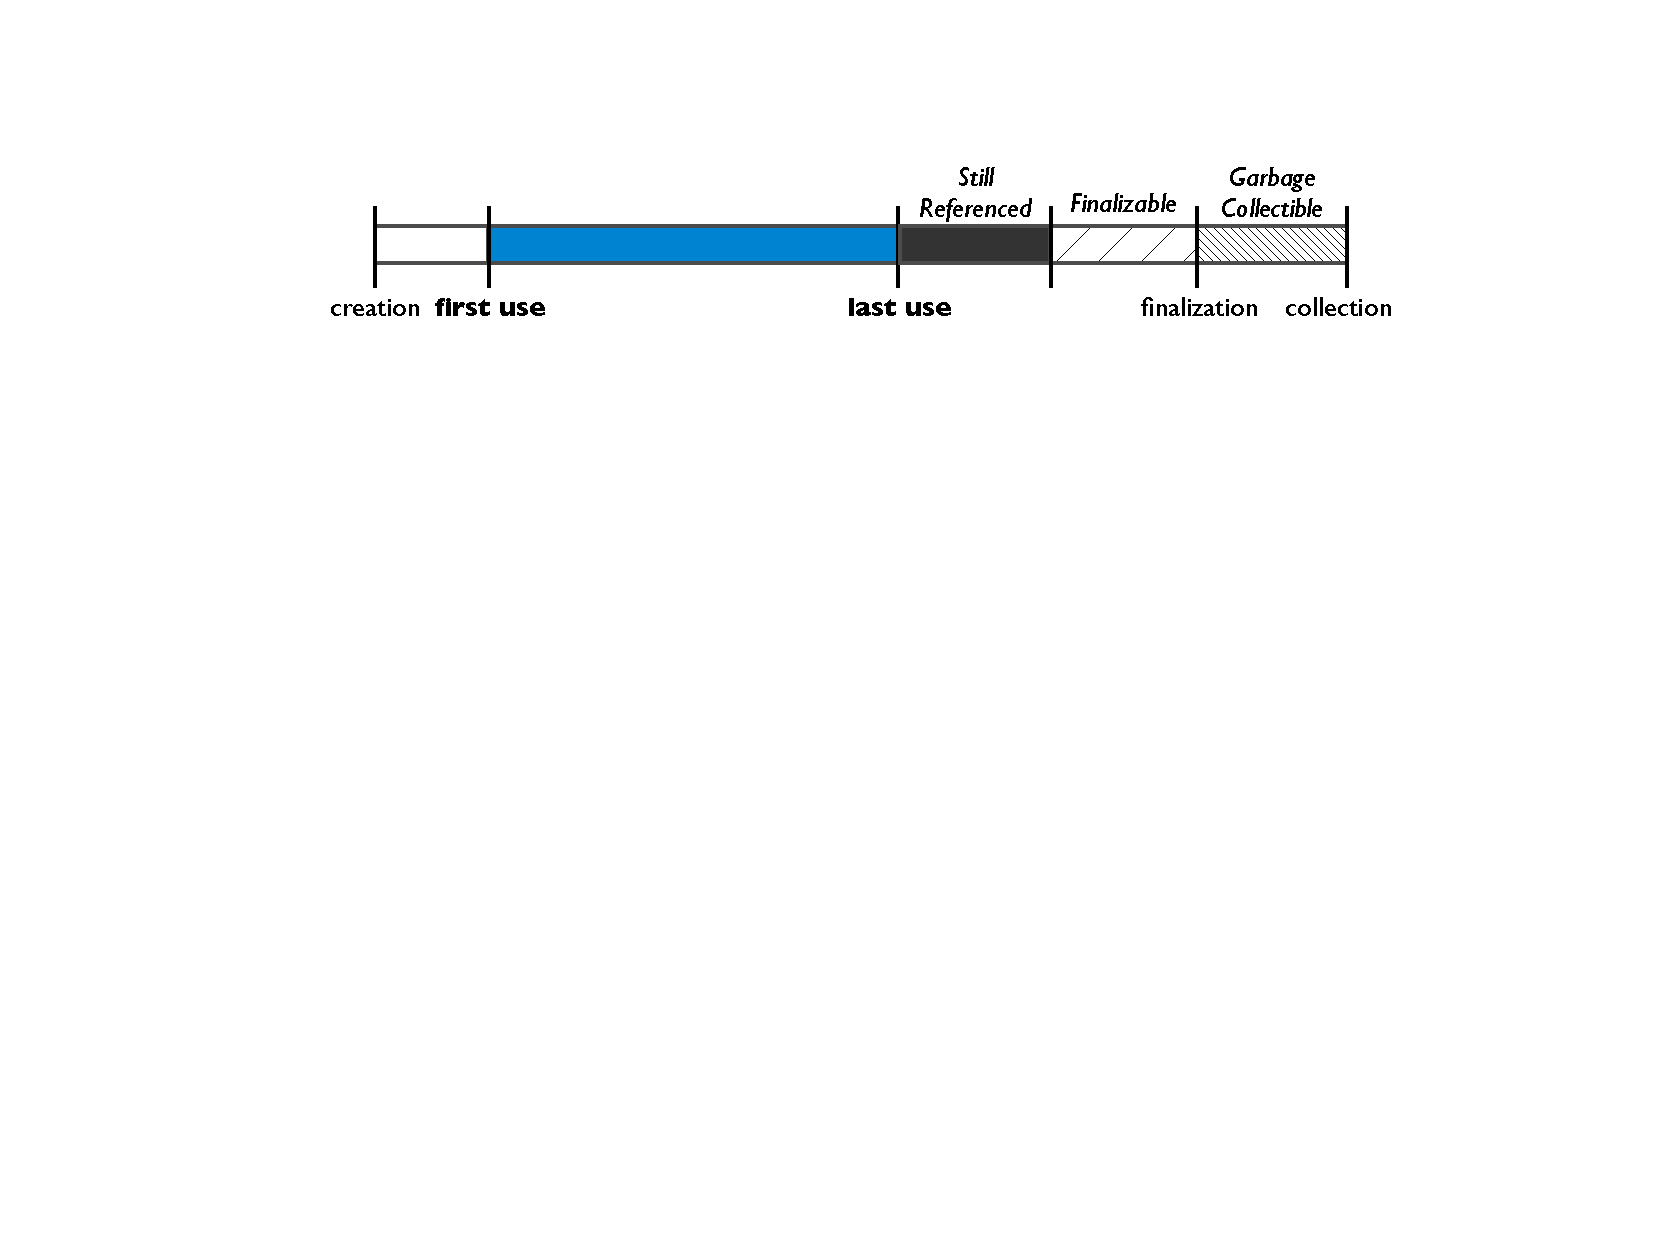
\includegraphics[width=0.9\textwidth]{part2/Figures/lifetime/object-lifecycle}
	\caption{Timeline of the life of a typical object.}
	\label{fig:typical-lifecycle}
\end{figure}


\begin{example}{Parsing a Date} Consider a loop that shows an easy way to parse
a list of dates. What objects are created, and what are their lifetimes?
\begin{shortlisting}
for (String string : inputList) {
	ParsePosition pos = new ParsePosition(0);
	SimpleDateFormat parser = new SimpleDateFormat();
	System.out.println(parser.parse(string, pos));
}
\end{shortlisting}
\end{example}

For each iteration of this loop, this code takes a date that is represented as a
string and produces a standard Java \class{Date} object. In doing so, a number of
objects are created. Two of these are easy to see, in the two \code{new} calls
that create the parse position and date parser objects. The programmer who wrote
this created two objects, but many more are created by the standard libraries to
finish the task. These include a calendar object, number of arrays, and the
\class{Date} itself. None of these objects are used beyond the iteration of the
loop in which they were created. Within one iteration, they are created, almost
immediately used, and then enter a state of drag.

\callout{drag}{Memory Drag}{
\index{Drag}
At some point, an object will never be used again, but the \jre doesn't yet know
that this is the case. The object hangs around, taking up space in the Java heap
until the point when some action is taken, either by the \jre or by the
application itself, to make the object a candidate for reclamation. The interval
of time between its last use and ultimate reclamation is refered to as
\emph{drag}.}

The \code{pos} object represents to the parser the position within the input
string to begin parsing. The implementation of the \code{parse} method uses it
early on in the process of parsing. Despite being unused for the remainder of the
parsing, the \jre does not know this until the current iteration of the loop has
finished. For this duration of time the object is in a kind of limbo, where it is
referenced but never be used again. This limbo time also includes the entirety of
the call to \code{System.out.println}, an operation entirely unrelated to the
creation or use of the parse position object. Once the current loop iteration
finishes, these two objects will become candidates for garbage collection.

\begin{figure}
	\centering
	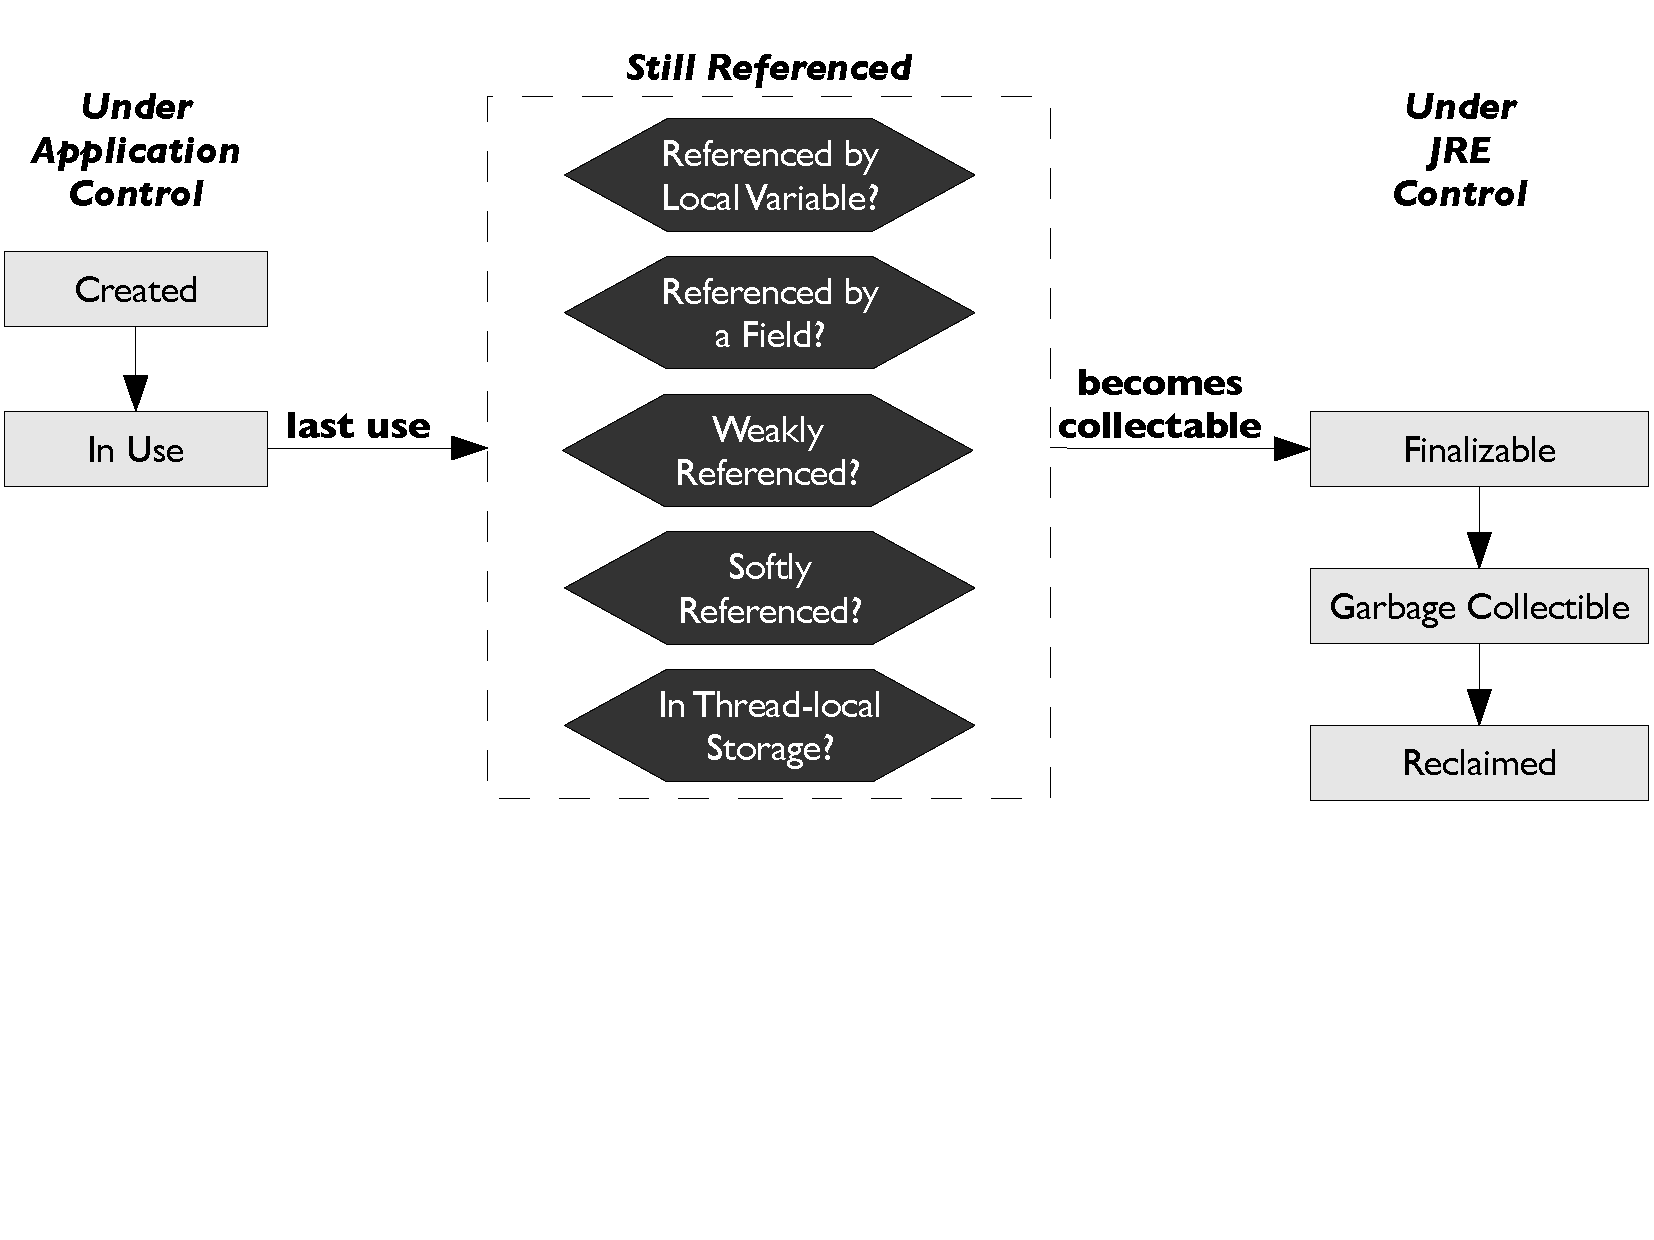
\includegraphics[width=\textwidth]{part2/Figures/lifetime/states}
	\caption{After its last use, an object enters a kind of limbo: the application
	is done with it, but it is not yet a candidate for garbage collection. When an
	object exits this limbo depends on the way it is referenced by your
	application.}
		\label{fig:limbo-exit}
\end{figure}

Depending on how the object is referenced by your application, it will
transition from in-use to garbage-collectable in a different manner. There are
eight ways an object may be referenced. It can be referenced by a:

\begin{enumerate}
  \item local variable of a method
  \item static field of a class
  \item instance field of a \class{java.util.ref.WeakReference} object
  \item instance field of a \class{java.util.ref.SoftReference} object
  \item instance field of a \class{java.util.ref.PhantomReference} object
  \item \tls
  \item instance field of any other object
  \item some combination of the above
\end{enumerate}

The first seven are cases of unique ownership of an object. There exists
only one path, via that particular reference, to reach the object. The eight case
is one of \emph{shared} ownership. After your program creates an object, it
references the object in one or more of these eight ways. The ownership of an
object may vary over time --- as your program runs, these references will come
and go. After some time, program execution may reach a point where the object is
no longer under application control. At this point, the \jre is now in charge of
its lifetime. For example, if the only reference to an object is from a field of
some other object, and your code reassigns that reference to \code{null}, this
becomes a point of transition, from application control to \jre control. Each of
the eight ways of referencing an object comes with its own guidelines as to when
this transition occurs. \autoref{fig:limbo-exit} and \autoref{tab:limbo-exit}
summarize how an object transitions to \jre control. The following code gives
examples of these eight patterns of ownership:
\lstset{numbers=left,numbersep=12pt,numberstyle=\tiny\textsf}
\begin{shortlisting}
class Foo {
   void bar(Object argument) {
      Object localVariableReference1 = new ...;
      threadLocal1.set(argument);
      threadLocal2.set(new ...);
      localVariableReference1 = null;
      for (...) {
         Object localVariableReference2 = new ...;
         ...
      }
   }

   static Object staticField = new ...;
   Object instanceField = new ...;
   Reference weak = new WeakReference(instanceField);
   Reference soft = new SoftReference(instanceField);
   Reference phantom = new PhantomReference(instanceField);
   ThreadLocal threadLocal1 = new ThreadLocal();
   ThreadLocal threadLocal2 = new ThreadLocal();
}
\end{shortlisting}
\lstset{numbers=none}
% Still, one can't always rely on automatic mechanisms to guide an object out of
% limbo in a timely fashion.

\begin{table}
\centering
	\begin{tabular}{ll} \toprule uniquely owned by  & 
	when object becomes candidate for reclamation \\ \cmidrule(r){1-1}
	\cmidrule(l){2-2}
			%
			nothing & immediately
        	\\
        	%
        	local variable & after scope exits, e.g. method returns
        	\\ \addlinespace
        	%
        	instance field of an object & 
        	when that object becomes reclamation candidate
        	\\
        	%
        	static field of a class &
        	when that class is unloaded
        	%
        	\\ \addlinespace
        	field of \class{WeakReference} & immediately
        	%
        	\\
	       	\ldots with \class{ReferenceQueue} &
        	immediately placed on queue, then after queue is polled
        	%
        	\\ \addlinespace
        	field of \class{SoftReference} & approximately
        	LRU%$^{**}$
        	%
        	\\
	       	\ldots with \class{ReferenceQueue} &
        	after LRU, placed on queue, then after queue is polled
        	%
        	\\ \addlinespace
        	entry in \tls & when that thread dies
        	%
        	\\ 
        \bottomrule
    \end{tabular}
	\caption{When an object becomes a candidate for reclamation. The dominating 
	reference can be explicitly overwritten, e.g. by your code expliclty assigning the
	reference to \code{null}. Otherwise, an object only automatically becomes a
	candidate under the restricted circumstances shown here.
%	The point when an object exits limbo depends on 
	%decisions under programmer control: it depends on how the object is
	%referenced.
	%older {\jre}s	use very poor heuristics for handling soft references; see the
	% body for more detail.
	%, it will be reclaimed
	%under certain rules, or may be part of a memory leak
	}
	\label{tab:limbo-exit}
\end{table}

\paragraph{The Lifetime of Local Variables}
\label{sec:lifetime-of-locals}
Variables that are declared within a method body often have a lifetime that is
bound to, at most, the duration of an invocation of that method.
% If an object is uniquely owned by a local variable of a method, the \jre will
% begin to consider reclaming its storage no sooner than when the local
% variable's scope exits.
Common examples of this are local variables, loop variables, and variables
declared within some inner scope such as within the body of a loop or \code{if}
statement. For these variables, when a loop continues to the next iteration as in
the case of \code{localVariableReference2}, when the body of a clause of an
if/then/else statement finishes, or when the method invocation returns as in the
case of \code{localVariableReference1}, there is a good chance that the object
referenced by that variable will be reclaimable.

There are situations where an object may \emph{escape} the local scope in which
it was declared.\index{Escaping Objects} In these cases, the object has
\emph{shared ownership}\index{Shared Ownership} until this local scope exits.
See below for further discussion of shared ownership. This is an example of an
object escaping a local variable scope, so that it is, for the duration of that
local scope, also owned by a static field of a class object:
\begin{shortlisting}
class Foo {
   static Object static_obj;
   
   void foo() {
      Object obj = new Object();
      static_obj = obj;
      ... // uses of obj
   } // obj scope exits, but static_obj ownership persists
}
\end{shortlisting}
The next section discusses the lifetime of static fields.

The minimum that the Java language specification requires is that non-escaping
objects that are declared within some scope inside of a method will be
reclaimable by the time that scope exits. Many modern \jres try to optimize by
inferring, when they can, the line of code at which an object will certainly
never be used again. For this reason, some (but not all!) sources of memory
drag\index{Drag} that would have been a problem with older \jres, are no longer
an issue. For example, you can run this test program and, by inspecting the
output, determine whether your \jre is performing this kind of optimization:
\begin{shortlisting}
/* Test for whether the optimizer detects that obj is reclaimable before the end of this method */
static public void main(String[] args) {
   Object obj = new Object() {
      protected void finalize() {
         System.out.println("Finalized");
      }
   };
   System.out.println("StartOfLoop");
   for (int i = 0; i < 1000000; i++) {
       new HashSet().add(i);
   }
   System.out.println("EndOfLoop");
}
\end{shortlisting}
If you see the \code{Finalized} message before the end of loop message, this is a
sure sign that the \jre is being clever. Be careful to remember that seeing the
finalized message is definitive evidence, but not seeing that message might only
mean that your loop doesn't iterate enough times to cause a garbage collection to
occur. You may need to experiment with the number of loop iterations, before
coming to a conclusion.

\paragraph{The Lifetime of Statics, and Class Unloading}
\index{Class Unloading}
\index{Static fields}

The \jre allocates memory for every class, to store its static fields, such as
the one on line 13 in the above example. This memory, to store all static fields
plus some bookkeeping information, is often referred to as the \emph{class
object} for the class.\index{Class Objects} It is possible for the same class to
be loaded into multiple class loaders; in this way, using more than one class
loader lets you avoid the problem of colliding use of static fields in separately
developed parts of the code. A static field therefore only exits scope when the
class object is reclaimed, which occurs when the respective class is unloaded, by
the \jre, from its class loader. 

If a class is never unloaded, which is likely to the be case for your
application, then that class object will remain permanently resident. The
\emph{default} class loader, which is the one that will be used unless you
specify otherwise, never unloads application classes. 

If you need classes to be unloaded, then you must manually specify a class loader
to use. Unloading a class is then accomplished by ensuring that all references to
both the class object and your custom class loader, are set to \code{null}. This
will render the class unloadable, and will also render objects referenced by
static fields all classes loaded into that class loader as garbage collectable.
There exist module management systems, such as OSGi~\cite{OSGi_2007}, that
facilitate this task.

Due to these complexities, your design should generally anticipate that the
memory for these static fields is permanently resident. This means that any
static fields referencing an instance, rather than containing primitive data,
will render that instance also permanently resident. Unless, that is, you take
action to explicitly clip the static field reference, by assigning the field to
null. Otherwise, that instance will be forever reachable along a path from some
garbage collection root through the static field reference. In this way, storing
a reference in a \code{static} field of an class is one way to implement a
permanently resident lifetime policy.

\paragraph{The Lifetime of Instance Field References}

As long as an object \code{B} is dominated by an instance field of another object
\code{A}, then these two objects will live and die together. The only device at
your disposal to make \code{B} garbage collectable before \code{A} is to break
all paths of references from \code{A} to \code{B}. In simple cases, where
\code{B} is directly referenced by a field of \code{A}, then reassigning that
reference to \code{null} will do the trick. After doing so, the \code{B} object
will now be a candiate for garbage collection. 



%Every object created by your application lives for an interval of time from its
%creation to the point that the Java runtime gets around to collecting it. An object's {\em natural} lifetime is defined by the
%interval of time between its first and last necessary use. %cite drag paper
%here?








\begin{comment}
\begin{figure}
	\centering
%	\subfigure[The lifecycle of a typical object and its data.]{
	%\label{fig:typical-lifecycle1}
			%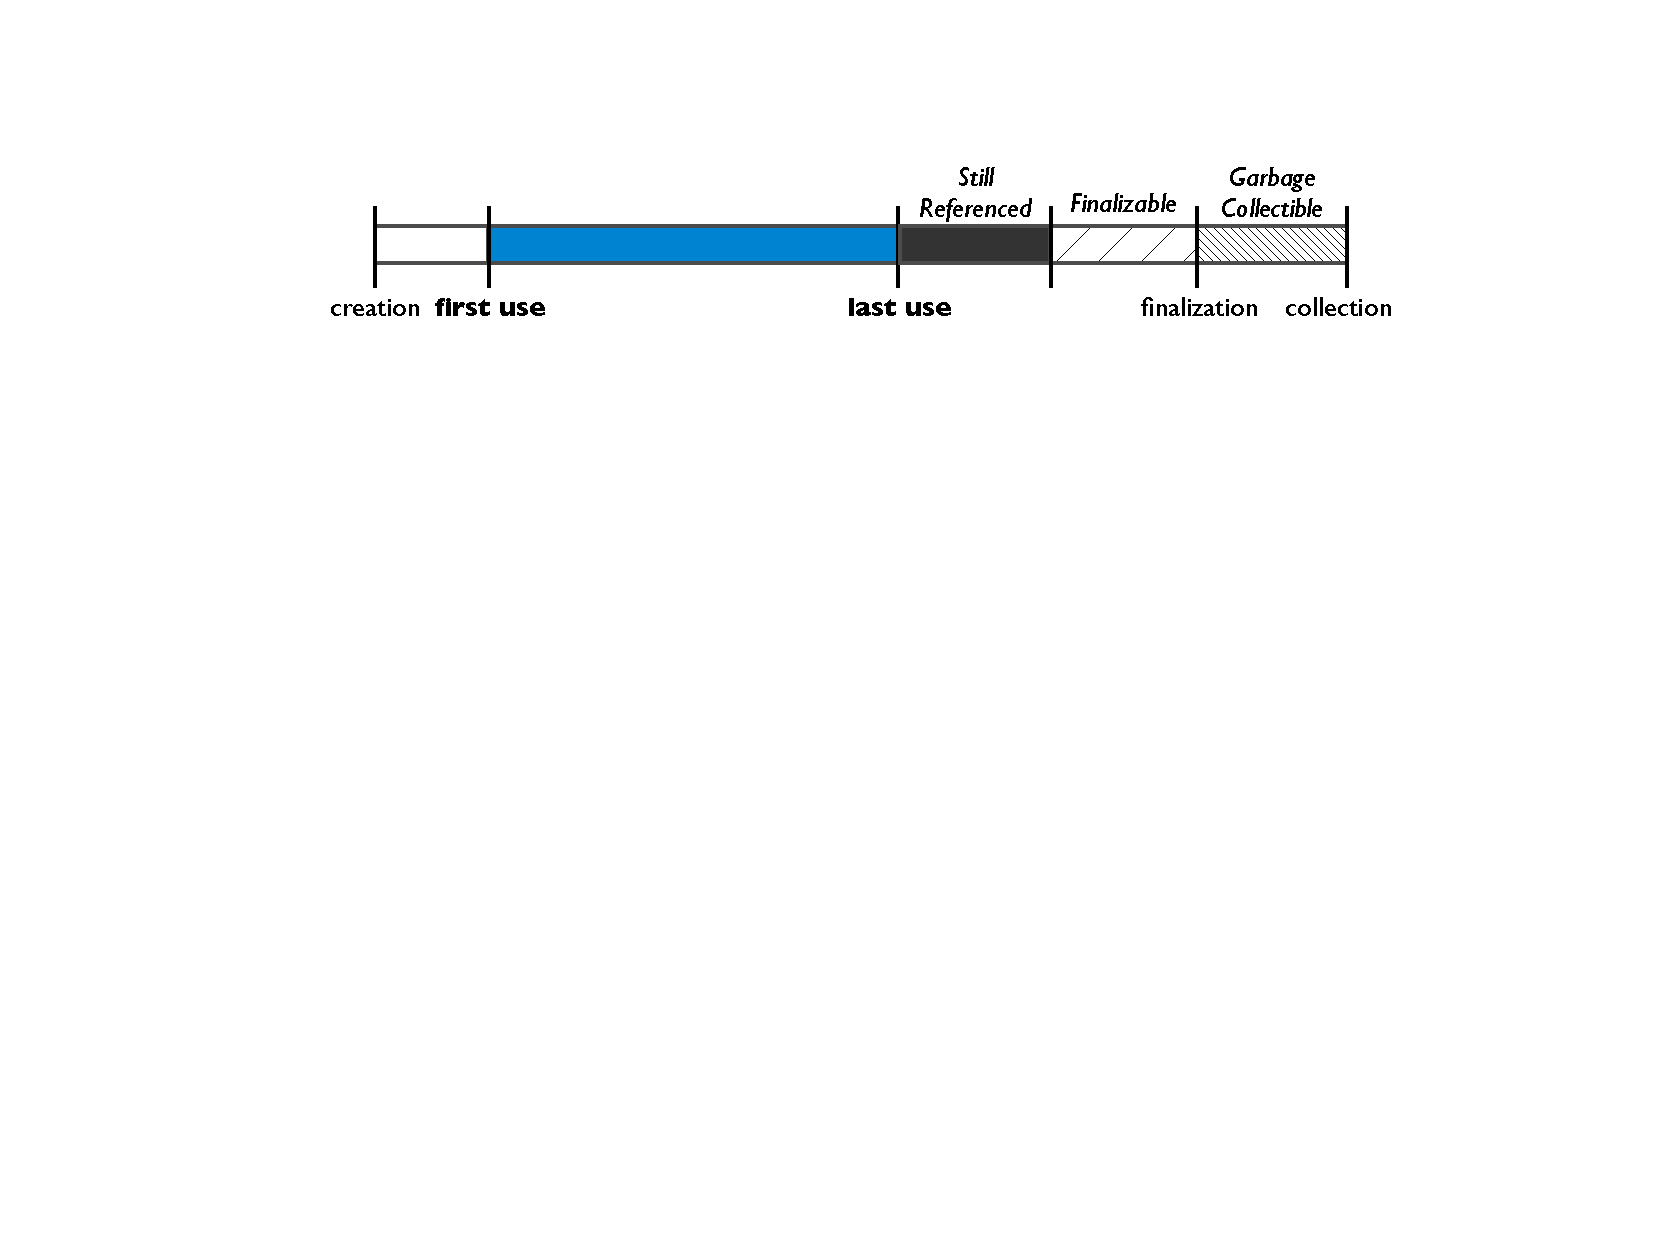
\includegraphics[width=0.95\textwidth]{part2/Figures/lifetime/object-lifecycle}
	%}
	\subfigure[A situation where there are long periods between uses of an
	object's data.]{
	\label{fig:typical-lifecycle2a}
		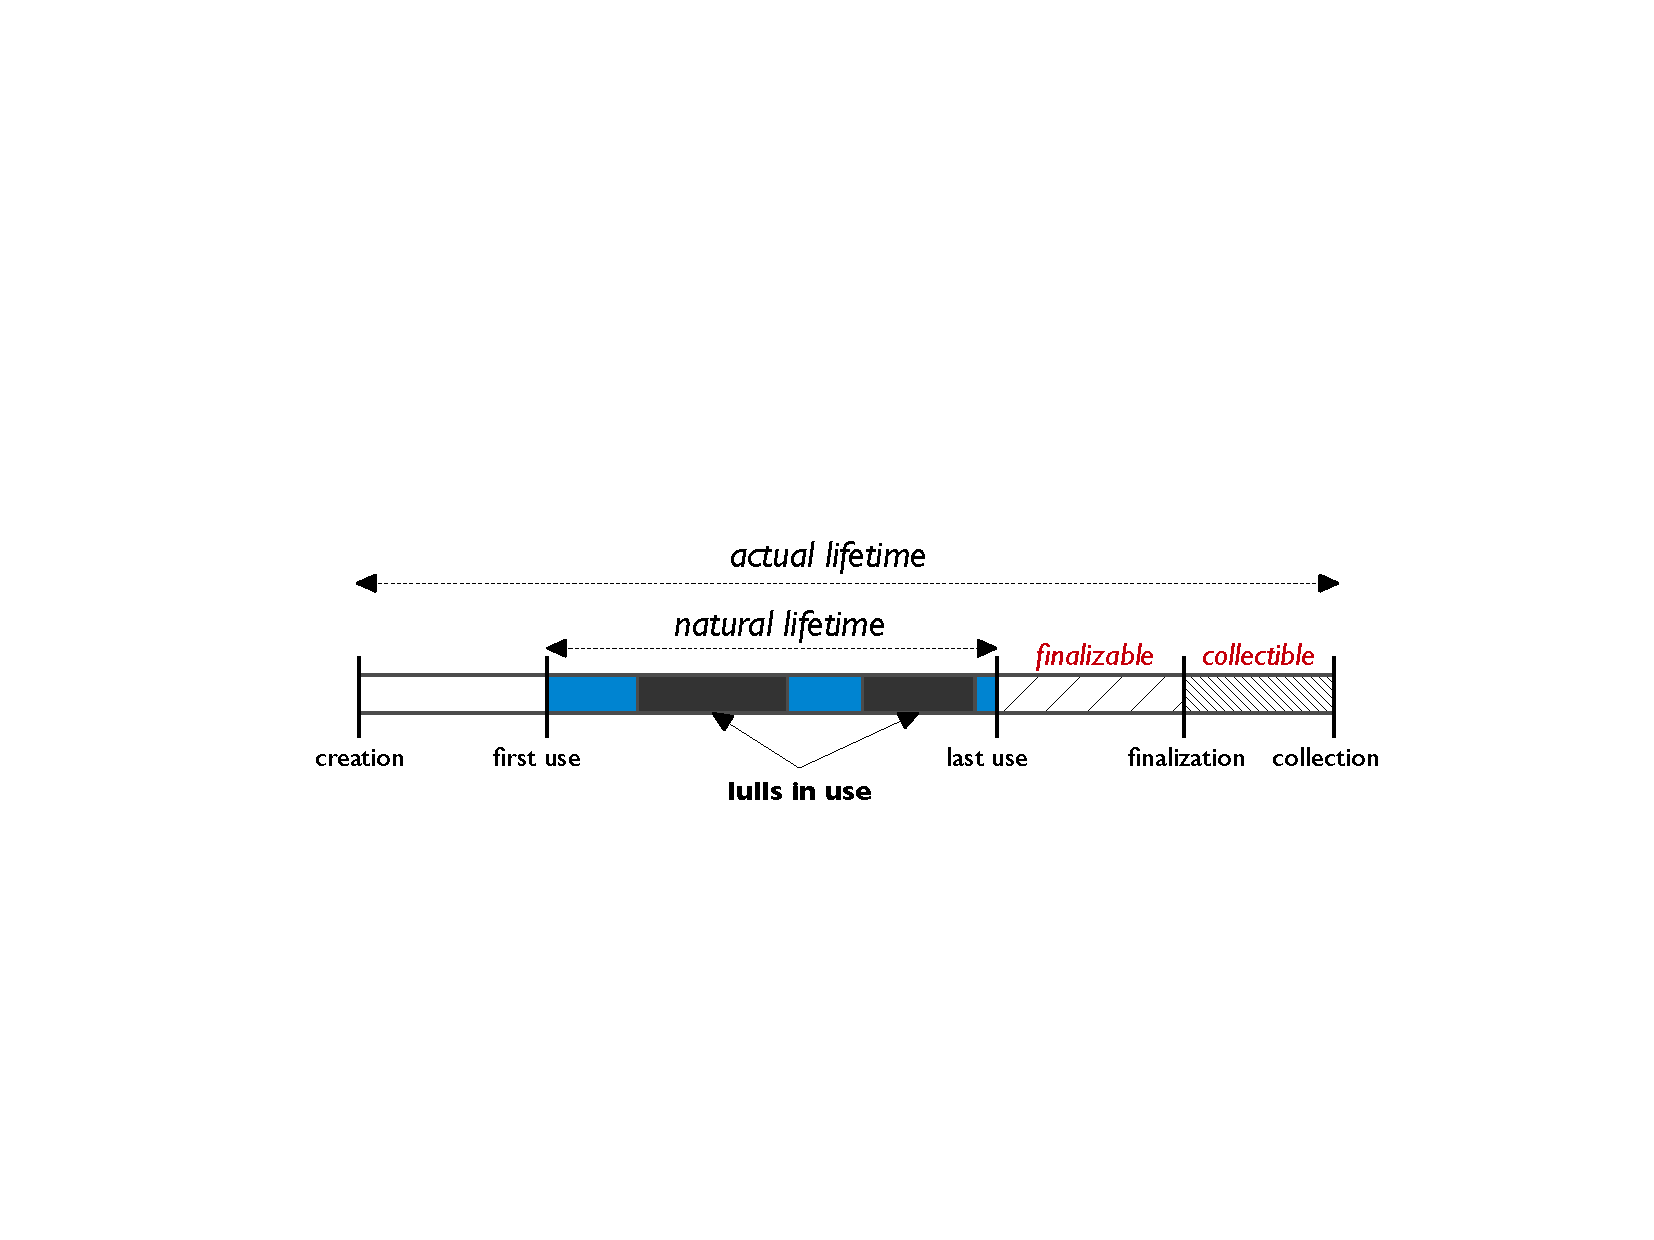
\includegraphics[width=0.95\textwidth]{part2/Figures/lifetime/object-lifecycle-lulls}
	}
	\subfigure[The lifecycle of the data  that is loaded from
	disk three times, and the objects that store it.]{
	\label{fig:typical-lifecycle2b}
		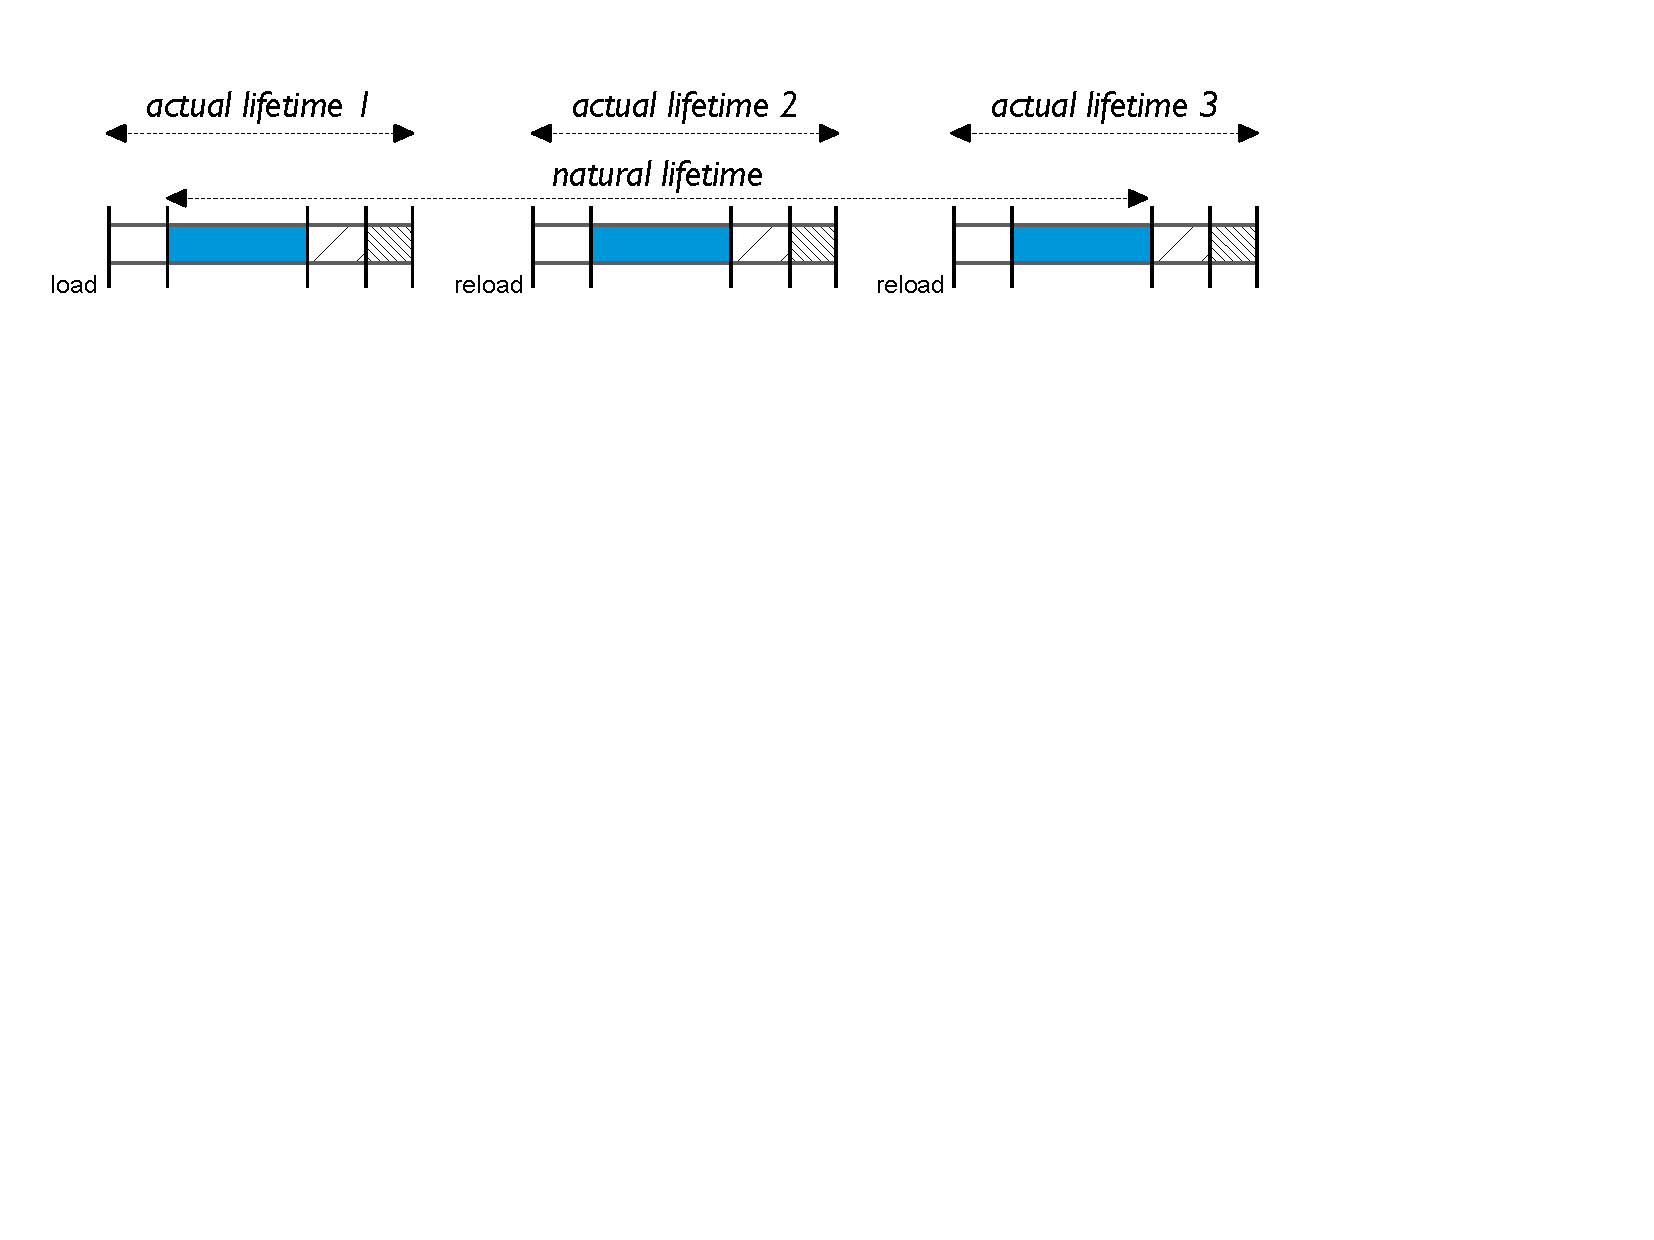
\includegraphics[width=0.9\textwidth]{part2/Figures/lifetime/object-lifecycle2}
	}
	\caption{Examples of Natural and Actual lifetimes.}
	\label{fig:typical-lifecycle2}
\end{figure}
\end{comment}


\paragraph{Shared Ownership}
\label{sec:shared-ownership}
\index{Shared Ownership}

When you invoke a library method, there is no way in Java to know what the called
method does with your object. It could very well squirrel away a reference to any
object reachable from arguments you pass to the invocation. Despite your best
efforts at keeping track of which references exist to an object, it can easily
become an uncontrolled mess once you pass these objects to third-party libraries.
In the above example, if you call the \code{parse} method of a
\class{SimpleDateFormat} object, the method contract says nothing about how it
treats the given string or \class{ParsePosition} passed as parameters. 
Consider the case where you need the string to become garbage collectable soon
after having parsed it, but the formatter maintains a reference in order to avoid
reparsing the same string in back to back calls. This calls
to mind the worst of the days of explicitly managing memory in a language like C.

In the case where there is more than one reference to the object, the story gets
more complicated. In contrast to C, where a \code{free} of \emph{any} pointer
suffices for deallocation, in Java \emph{all} references to an object must be
assigned to \code{null}. This is tricky in many cases, because it may not be easy
to know where all those references emanate from.
\autoref{fig:reachability-sharing} illustrates a situation where three references
must be clipped before an object, the darkly shaded one, becomes a candidate for
garbage collection. There are two other important things to note in this example.
First, just as in \autoref{fig:reachability-b}, after clipping the three
indicated references, an entire data structure, not just that darkly shaded
object, becomes a candidate for reclamation. This structure consists of the two
objects contained within the lightly shaded region. The second important thing to
note is that you needn't clip the backwards edge, or any edge contained entirely
within the data structure you no longer need.

\begin{figure}
\centering
\subfigure[Diamond sharing.]{
	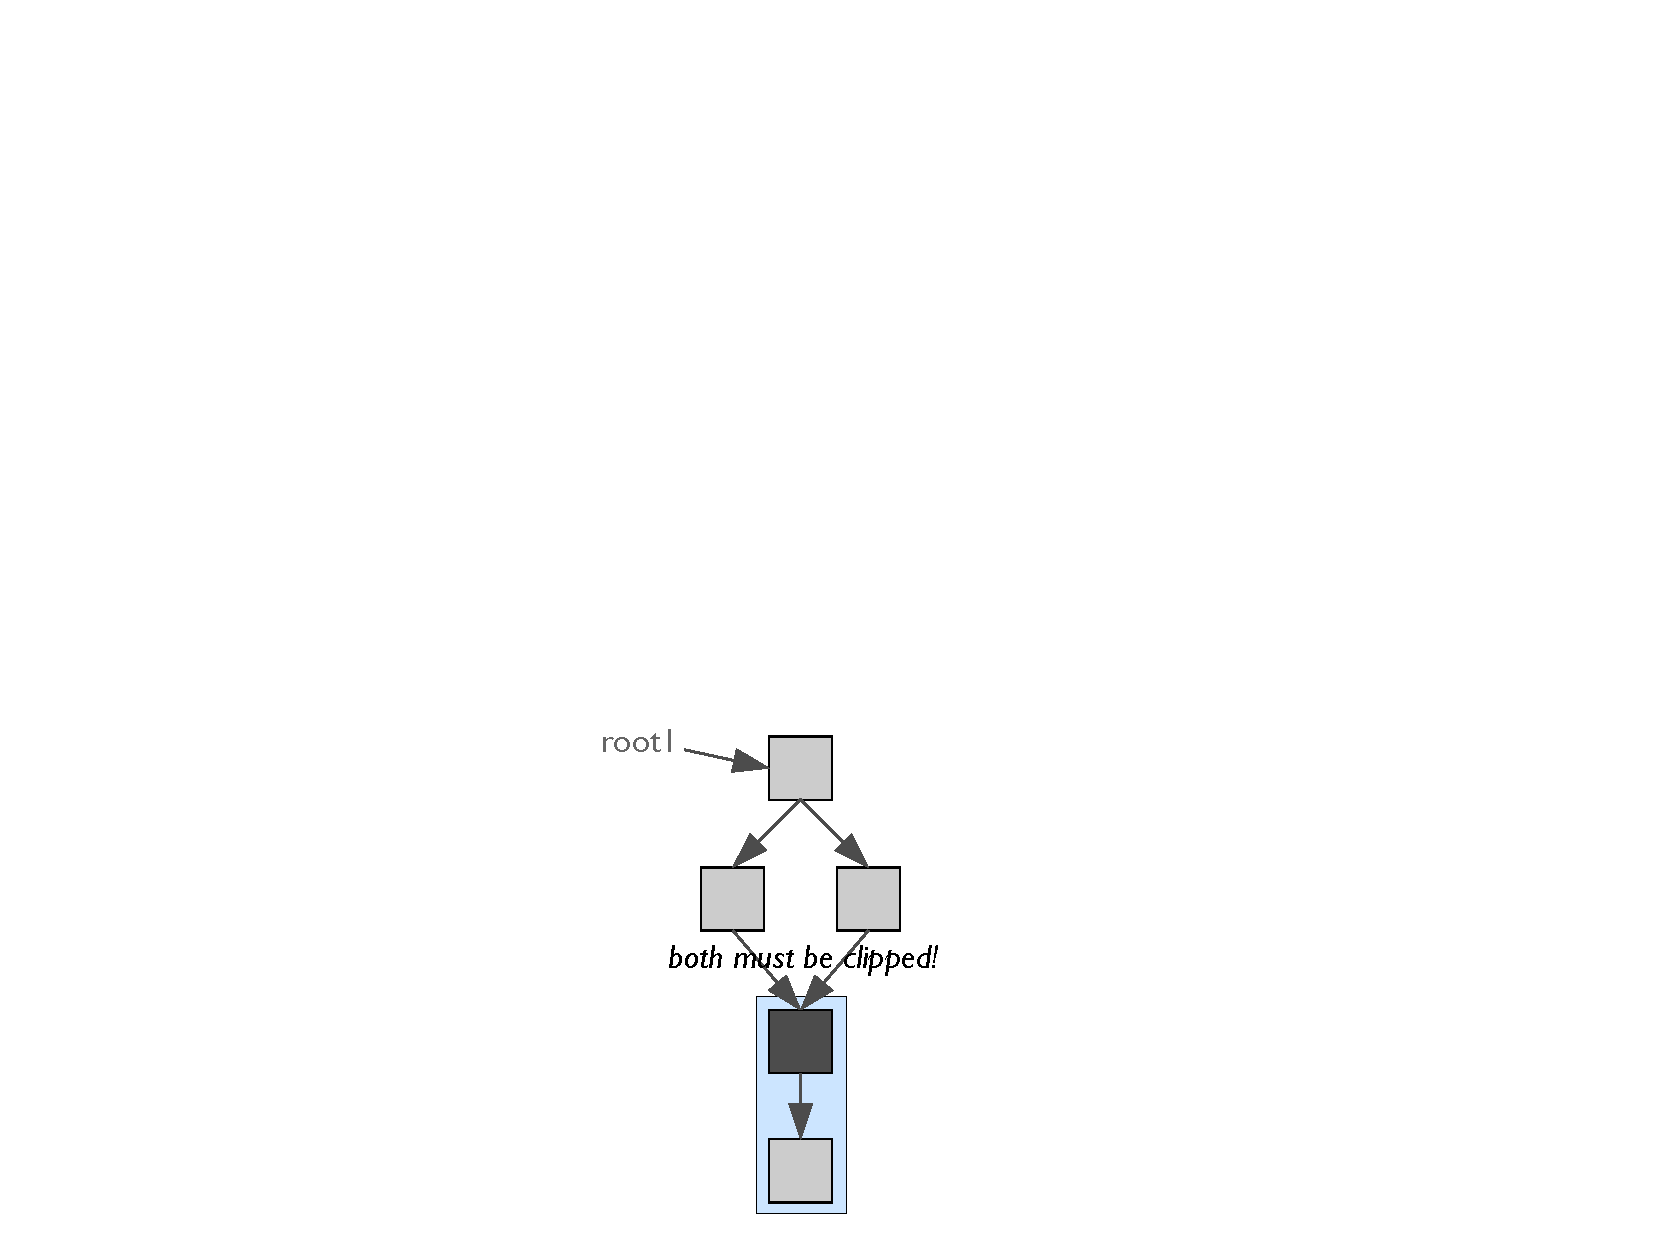
\includegraphics[height=0.25\textheight]{part2/Figures/lifetime/reachability4}
	}
\qquad
\subfigure[Root sharing.]{
	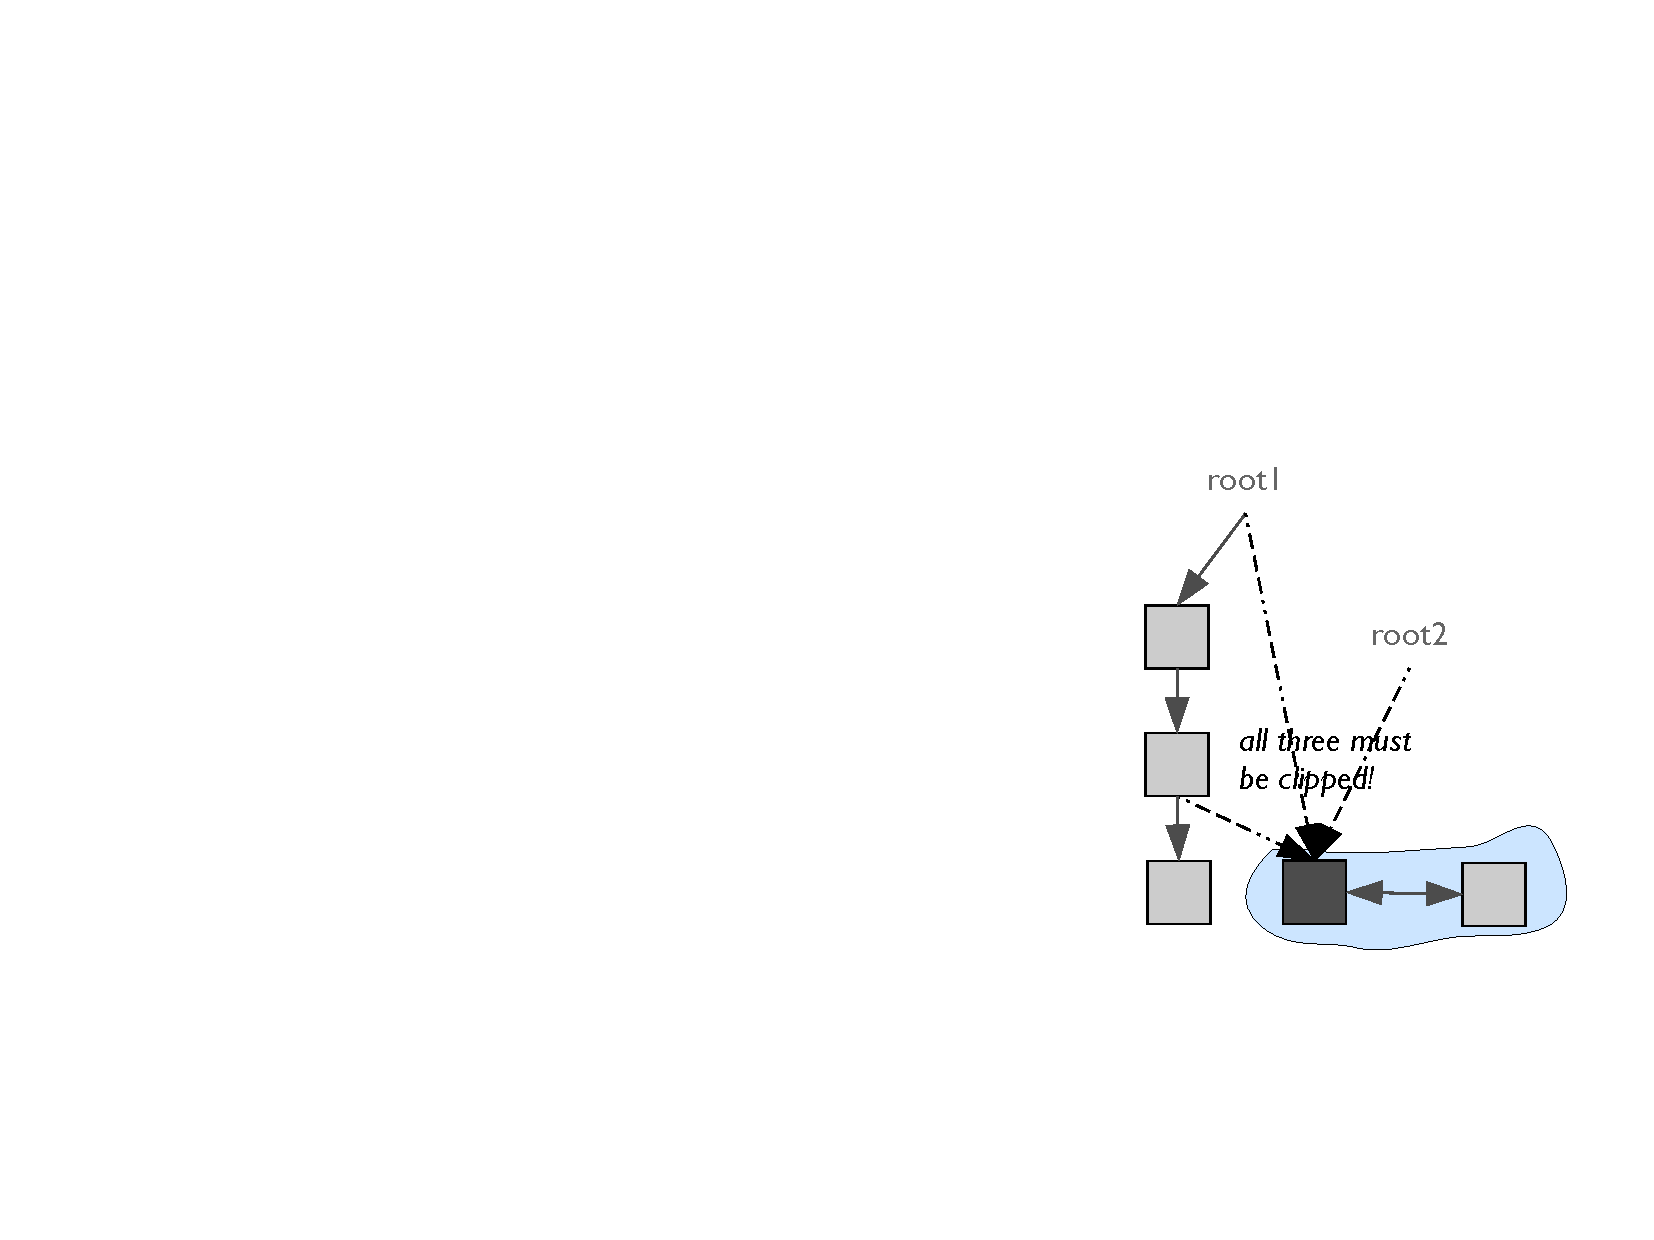
\includegraphics[height=0.22\textheight]{part2/Figures/lifetime/reachability3}
	}
	\caption{When an object is shared, such as the shaded ones shown
	here, care must be taken to clip all edges from emanating from outside of the
	region you wish to reclaim.}
	\label{fig:reachability-sharing}
\end{figure}

\section{Advanced Lifetime Management Features}
 
There are several important lifetime management policies that cannot be expressed
using normal mechanisms of local variables and static and instance field
references. For example, to implement the correlated lifetime policy described in
\autoref{sec:correlated-lifetime} using only the mechanisms presented so far is
difficult. In \autoref{fig:reachability-b}, there are three objects contained
within the shaded region; these three objects will all be garbage collectible if
the indicated dominating reference is set to \code{null}. In this way, the
lifetime of the lower two can be correlated with the lifetime of the object
directly pointed to by the dominating reference. This can work, in certain
limited circumstances, but it requires that you encode the correlation in the
class definition itself. To correlate an instance of the \class{B} class with an
instance of the \class{A} class, you must add a field to \class{A}:
\begin{shortlisting}
class A {
   B b;
}
\end{shortlisting}
In addition to requiring the pollution of class definitions, it also can result
in wasted memory. If only some \class{A} instances have a correlated \class{B},
then you will be wasting a pointer slot for every instance of \class{A}. It turns
out that this is how the Java standard \class{HashMap} was implemented, in its
mechanism for maintainin a correlation between the various views (the key set,
value set, and entry set), and the map itself:
\begin{shortlisting}
class HashMap {
   Set keySet, valueSet, entrySet;
}
\end{shortlisting}
This choice had a big implication on the memory bloat factor of small maps. As
we have learned in previous chapters, every instance of a standard Java hash map
must pay the expense for potential use of features. These features aren't
always employed, and certain rarely together, for a single map instance.

\paragraph{Weak and Soft References}
The Java language provides mechanisms that allow you more flexibility in
implementing lifetime management policies. These advanced features are exposed
via the \class{java.lang.ref.Reference} family of classes and \tls. Programmers
very often confuse these mechanisms, and there is quite a bit of disinformation
on the Internet; there is especially confusion over the use of soft and weak
references. Therefore, it is important for you to take some care in understanding
the low-level features.

To contrast the normal referencing mechanisms with these advanced features, the
normal ways of referencing objects are typically referred to as \emph{strong}
references. This term came about to contrast with the terms used for the more
advanced features: weak, soft, and phantom references.

\paragraph{Finalization and Phantom References}
\index{Finalization of objects}
\index{Phantom References}


\paragraph{\TLS}
\tlsindex % \index{\TLS} doesn't seem to work

\section{Summary}



\chapter{Implementation Practices for Sound Lifetime Management}
\label{chapter:lifetime-implementation-strategies}

Typically, objects die soon after the point in time of their last use, once all
dominating references are removed or naturally go out of scope. For a great many
objects, the normal flow of method invocations results in local variables going
out of scope, which renders these objects reclaimable without any special effort
on your part. In the absence of memory leaks, and without any optimizations,
objects live and die according to this \emph{natural lifetime}, as discussed in
depth in \autoref{sec:natural-lifetime}. 

However, the built-in lifetime mechanisms, by relying on objects going out of
scope, are insufficient to implement the more complicated patterns.
Implementations of the correlated lifetime pattern, introduced in
\autoref{sec:correlated-lifetime-pattern}, are very prone to memory leaks. You
may need an object to survive for a period of time that is not bound to any one
method invocation, but rather to the lifetime of another object. The lifetime of
some objects are indeed correlated with an invocation, as in the case of objects
correlated with a phase or request, but even here there are difficulties.
Oftentimes, the invocation that marks the beginning of a request is in a part of
the code outside of your control, or is distant from the allocation site of the
objects that must go away when the request finishes. Implementations of the
time-space tradeoff pattern, introduced in
\autoref{sec:time-space-tradeoffs-pattern}, can be ineffective if they aren't
sized properly. They, too, can result in memory exhaustion, e.g. if a cache's key
misimplement equality, or if it is sized too large.

It is important to code according to practices that will assure that an object
dies when it should. The correlated lifetime and time-space tradeoff patterns are
the most difficult cases to get right, and so those most in need of rigorous
coding practices.

% managing a reference queue

%\section{Lifetime Management Principles}


\section{The Sharing Pool Pattern}
\label{sec:sharing-pools}
\index{Sharing Pool}

\marginpar{A \textbf{Sharing Pool} stores canonical instances of data values that
would otherwise be replicated in many objects.} It is very common for
applications to store many copies of the same data in multiple data structures.
This is especially a problem with strings. Heaps can often store the same string
dozens or even hundreds of times. The sharing pool pattern is a way to amortize
the memory cost of data over many uses of it that overlap in time. If they don't
overlap in time, then you might still find it beneficial to amortize the
construction time, but this is a different lifetime pattern. It is a time-space
tradeoff, rather than a space-reduction optimization; see the resource pool
pattern below.

The general shape of the solution lies in a \emph{canonicalizing map}, one that
maps a new data structure to a previously constructed data structure with the
same shape and data values. Once you have made the decision to extend the
lifetime of an object, of those canonical instances, you have introduced a
lifetime management problem.


\begin{example}{Duplicate Strings}
You application loads data from a file. This data contains a large number of
name-value maps that will be used frequently throughout program execution.
These maps represent configuration information. The names come from a small set
of 16 distinct names. The set of string values 
is unknown at development time, but is known to be small;
you know there aren't going to be many distinct values, but you are unwilling or
unable to nail them down at compile time. How can these maps be stored in a memory
efficient way?
\end{example}

Without any special effort, each instance of this kind of configuration map
would store the some subset of same 16 key strings. Furthermore, each map would
store duplicates of the values. The following code snippet has those two
aspects of duplication:

\begin{shortlisting}
Map<String,String> map = new HashMap<String,String>();
void handleNextEntry() {
   String key = getNextString();
   String value = getNextString();
   map.put(key, value);
}
\end{shortlisting} 

Java provides a built-in mechanism for sharing the contents of strings across
many string instances. By \emph{interning}\index{String interning} a Java
\class{String}, you ensure that the returned \class{String} will only have
distinct storage if it is a string value that hasn't been interned yet. You can
modify the first try as follows:

\begin{shortlisting}
void handleNextEntry() {
   String key = getNextString().intern();
   String value = getNextString().intern();
   map.put(key, value);
}
\end{shortlisting} 

It is possible to do even better, if you have the luxury of modifying both ends
of the communication channel, i.e. both the serialization and this
deserialization code. There are only 16 distinct names used in all instances of
this configuration map. This seems like a perfect case for an enumerated type. An
enumerated type can be used to represent strings as numbers at runtime. The only
place the strings are stored is in the string constant pool\index{Java's Constant
Pools}. Each class, when compiled, keeps a pool of the strings that are used by
code in that class. In this way, an enumerated type is an even more highly
optimized sharing pool than that provided by the interning mechanism. 

Enumerated types offer an additional opportunity for decreased memory bloat.
Since, in this example, the keys can be represented as an enumerated type, you
can use the \class{EnumMap} to store the mapping. It is over 3 times as space
efficient as a \class{HashMap}, consuming only 28 bytes per collection and 8
bytes per entry compared to 120 bytes per collection and 28 bytes per entry for a
\class{HashMap}.

\begin{shortlisting}
enum PropertyName = {...};
Map<PropertyName,String> map = new EnumMap<PropertyName,String>(PropertyName.class);
void handleNextEntry() {
   PropertyName key = getNextPropertyName();
   Object value = getNextString().intern();
   map.put(key, value);
}
\end{shortlisting} 

There is an important variant of a sharing pool called the Bulk Sharing Pool.
Like a normal sharing pool, the goal of a bulk sharing pool is to amortize the
memor costs of storing data. However, rather than mitigate the costs of data
duplication, a bulk sharing pool aims to amortize the costs of Java object
headers across the elements in a pool. This is a topic that stretches notions of
how to store data beyond the normal Java box, and so will be discussed, along
with many similar matters, in \autoref{chapter:large-long-lived}.

\section{The Single Strong Owner Pattern}

Lifetime management for temporaries (the lifetime pattern discussed in
\autoref{sec:temporary-lifetime}), and for objects that are part of only one data
structure at a time is usually pretty straightforward. The lifetime of a
temporary object, such as one created within a method and not used beyond the end
of the method, will be nicely governed by local variable scoping rules.

Many lifetime management bugs arise from shared ownership of non-temporary
objects. When an object that is simultaneously part of more than one data
structure, as introduced in \autoref{sec:shared-ownership}, it becomes hard to
keep track of what actions need to be taken in order to make that object
reclaimable by the \jre. Even if you make your best effort to avoid this problem,
such as by using weak references, you can still have problems. The diamond
structures described in \autoref{sec:strongweakdiamonds} are a good example of a
case where, even with weak references, objects may stick around too long. What
programming patterns can help to avoid these problems, so that you aren't left
hunting down hard to diagnose memory leaks late in the development lifecycle?

Ideally, every object would be part of only one data structure at a time. This
would simplify lifetime management issues, because there would be no hidden
links for you to track down and eliminate. This is of course not possible in any
practical setting. It is necessary for multiple, probably unrelated, parts of
the code to need access to a common set of objects. The listener pattern,
covered in more detail below, is a common case of this. For example, in user
interface code, both the callback handler for user events and the redraw loop
will operate on the underlying data model that the view exposes.

A more practical spin on this single-owner ideal is that every object
should have a \emph{home base}.
\callout{home-base}{The Home Base as Single Strong Owner}{
%A good design principle is to consider that every object, 
If an object simultaneously is part of
multiple data structures, then identify one of these as its \emph{home base}.
The home base data structure should be the \emph{single strong owner} of this
shared object. Every other data structure must only weakly or softly reference the
object.}

For example, consider an object that is part of a cache. While it is not in use,
the cache is the sole owner of the objects. If it weren't for the cache holding
a non-weak reference to the object, it would be reclaimed. When a cached object
is being used by the program, it will likely also be part of other data
structures; these structures may possibly span multiple threads. The cache is a
natural home base, and any other transitory owners of the objects msut be
designed so that their ownership is indeed transient.

A first piece of implementing this single strong owner pattern is the home base
itself:
\begin{shortlisting}
class HomeBase {   
   Set owned = new HashSet();
   
   public void own(Object o) {
      owned.add(o);
   }
}
\end{shortlisting}

%\lstset{moredelim=[is][\underbar]{|}{|}}

On its own, the \class{HomeBase} class provides a repository for strong
references, but doesn't help much in assuring that it is the \emph{only} strong
reference to the objects.To add this extra level of assurance requires four
pieces of logic. First, you need to make sure that every other collection in
which these objects are placed does not have a strong reference to the object.
Second, it would be a big headache to have to call
\class{HomeBase.own()} on every object that you create. This would
heavily pollute your code and be a nightmare to maintain. You can combine the
first two, if there are facades for the collections that take care of the
registration process for you. Third, there are several important use cases for
which the collections are intended to hold data for multiple tasks. Therefore,
you can't simply associate one \class{HomeBase} repository with a
collection; e.g. you may have a single map that contains data for multiple
tasks, each of which needs its own repository. The final issue is how to ensure
that the repository itself becomes reclaimable soon after you are done with it.
A rigorous coding practice is necessary to avoid holding on to the repository
itself for longer than necessary.

You can use a factory design pattern to help. The factory should have this basic
structure:
\begin{shortlisting}
class HomeBaseFactory {
   public HomeBase newOwner() {
      return new HomeBase();
   }

   public Map newMap(HomeBase home) {
      return new WeakHashMap() {
         public Object put(Object key, Object value) {
            home.own(key); return super.put(key, value);
         }
      }
   }
}
\end{shortlisting}
In this base implementation, the \code{newOwner} method doesn't do anything
fancy. But it does provide factory methods for creating a map facade that takes
care of associating ownership with a given repository, while keeping the map
itself free of eternally persistent references to the map's contents. Once the
repository is reclaimed, then the weakly referenced key will be reclaimed, at
which point, or shortly thereafter, the \class{WeakHashMap} will take care of
removing the entire entry (see \autoref{sec:weakhashmap}). From this base
implementation, it should be easy for you to implement similar factory methods
for the other kinds of collections, such as sets and lists.

It is often the case that the repository for ownership can reside within a
thread. If so, you can leverage the \tls mechanism to implement
a factory that provides unique ownership respositories
\begin{shortlisting}
class ThreadLocal_HomeBaseFactory extends HomeBaseFactory {
   ThreadLocal<HomeBase> threadLocals = new ThreadLocal<HomeBase>();
   
   protected void own(Object o) {
      // the thread's HomeBase assumes ownership
      return threadLocals.get().own();
   }

   public HomeBase newOwner() {
      HomeBase home = new HomeBase();
      threadLocals.set(home);
      return home;
      // the caller will now have the only strong reference to the HomeBase repository, we maintain only a weak reference to it
   }
}
\end{shortlisting}

But this implementation suffers from memory drag. After the thread's task
completes, the \tls maintains a reference to the \class{HomeBase} and
all the owned objects. It will only be overwritten either when the same thread is
scheduled to process a new task, or when the thread terminates. You could
overcome this by adding a \code{clear} method, and inserting a call to it at the
right place in your code:
\begin{shortlisting}
public void clear() {
   threadLocals.set(null);
}
\end{shortlisting}
However, this is a messy and error prone solution. An alternative solution is to
rely on local variable scoping to automatically clean things up for you. When a
task begins, you can grab a strong reference to the \class{HomeBase}
repository, and have the \tls maintain only a weak reference to
it:
\begin{shortlisting}
class ThreadLocal_HomeBaseFactory extends HomeBaseFactory {
   ThreadLocal<WeakReference<HomeBase>> threadLocals = new ThreadLocal<WeakReference<HomeBase>>();
      
   protected void own(Object o) {
      // the thread's HomeBase assumes ownership
      return threadLocals.get().get().own();
   }
   
   public HomeBase newOwner() {
      HomeBase home = new HomeBase();
      threadLocals.set(new WeakReference(home));
      return home;
      // the caller has the only strong reference to the HomeBase repository, we maintain only a weak reference to it
   }
}
\end{shortlisting}
Now, all objects owned by the repository will be automatically reclaimable when
the return value of \code{newOwner} goes out of scope.

%\subsection{Safety Valves}

%\section{Example Applications of Lifetime Practices}
\section{The Correlated Lifetime Patterns}

Implementing a correlated lifetime pattern in a way that does not result in
memory drag or memory leaks is difficult. There are four important cases:
annotations, annotation pools, listeners, and phase/request-scoped objects.

\subsection{Annotations}

If you don't have the luxury to change a class definition, but need to associate
some information with it, then your only choice is to use a map. To ensure that
the lifetime of the annotation is correlated with the lifetime of the annotated
object, you can use a \class{WeakHashMap}. \autoref{sec:weakhashmap} introduced
this utility class, that is part of the standard library. For example, to
associate a class \class{A} with a class \class{T}:

\begin{shortlisting}
class AnnotationMap<T,A> extends WeakHashMap<T, A> {
   public void annotate(T t, A a) {
      super.put(t, a);
   }
}
\end{shortlisting}

This implementation works well, at least for single-threaded programs. Soon after
an annotated T instance is reclaimed, the \class{WeakHashMap} will automatically
take care of removing the annotation entry from the map. If your application has
multiple threads concurrently accessing and creating these annotations, then you
will suffer from lock contention.
\autoref{sec:lifetime-management-concurrency-issues} discusses solutions to this
problem.

There is a more immediate potential problem, however. If your annotations are
more than simple objects like dates, then you have to be very careful to avoid
the strong-weak diamond problem described in \autoref{sec:strongweakdiamonds}.
This problematic situation can arise if an annotation, either directly or via
some chain of fields, strongly references the annotated object. This is a common
and innocent mistake, when you code in a way that avoids the messiness of
creating a reverse lookup map, from annotations to annotated objects:
\begin{shortlisting}
class TimestampAnnotation<T> {
   T t;
   Date date;
   
   public TimestampAnnotation(T t) {
      this.t = t;
      this.date = new Date();
   }
}
\end{shortlisting}
But this example will result in the annotation map leaking memory. You must have
the annotaitons weakly reference the annotated object, i.e. the \code{T t} field
must be replaced with a \code{WeakReference<T> t}. 
%Careful application of the
%single strong owner principle would help to avoid these mistakes. For example,
%you could offer a factory method 

%\begin{example}{Timestamp Annotation}
%How can you associate a timestamp with an object in a way that avoids memory
%leaks and that scales well to a highly concurrent workload?
%\end{example}
%
%We can start with the following code:
%
%\begin{shortlisting}
%class TimestampAnnotation<T> {
	%T t;
	%long timestamp;
%}
%List annotations;
%for (String string : inputList) {
	%...
	%annotations.add(new WeakReference(new Wrapper<String>(string)));
	%...
%}
%\end{shortlisting}
%
%Despite your use of \class{WeakReference}, you would find that neither the main
%object (the strings), nor the annotations, would ever be collected. This code
%has two memory leaks. One of the leaks is due to a
%violation of the first principal of the use of weak references: the annotations
%strongly reference the objects being annotated. It is not always this easy to
%debug problems in using weak references. Your application will hold on to
%objects that you didn't expect. Quite often, it is difficult to even know that
%there is a problem in the first place! The application may behave normally,
%except that it will consume more memory than necessary; if this extra memory
%consumption pushes it over your maximum heap size, then your application will
%crash --- you will know something is wrong, but diagnosing this type of
%problem, a memory leak\index{Memory Leak}, is quite difficult. It is better to
%keep the three principles of weak references in mind, and design in a way that
%avoids memory leaks in the first place. Your annotations can be modified to use
%a \class{WeakReference} to the main object:
%
%\begin{shortlisting}
%class TimestampAnnotation<T> {
	%WeakReference<T> t; // annotation only weakly refs main object
	%long timestamp;
%	
	%TimestampAnnotation(T t) {
		%this.t = new WeakReference(t);
	%}
%}
%\end{shortlisting}
%
%In this case, the annotation has no normal references to the annotated object,
%and so it obides by the first rule of weak references. If you remember from
%\autoref{chapter:delegation}, the code can be improved further to avoid the
%cost of delegation. This version of the annotation class extends
%\class{WeakReference}:
%
%\begin{shortlisting}
%class TimestampAnnotation<T> extends WeakReference<T> {
	%long timestamp;
%	
%	TimestampAnnotation(T t) {
		%super(t);
	%}
%}
%\end{shortlisting}
%
%Unfortunately, both of these updated versions h?
%%%%%%%
% old version??
%You could store the annotations in a map that is keyed by the
%original object, say of type \class{T}:
%
%\begin{shortlisting}
%Map<T, Date> timestamps = new HashMap<T, Date>();
%
%void addTimestamp(T t) {
	%timestamps.put(t, new Date());
%}
%Date getTimestamp(T t) {
%	return timestamps.get(t);
%}
%\end{shortlisting}
%
%This solution will function correctly, but suffers from a \emph{memory
%leak}\index{Memory Leak}. As the application runs, it will consume greater
%amounts of Java heap, up until the point when the \jre runs out of heap space
%to allocate any more objects. This solution leaks memory, because the
%\code{timestamps} map introduces a reference to the main objects. When the
%garbage collector scans the heap to see which objects are still alive, the
%references in this map will be among those that keep the objects alive. The
%next chapter discusses these issues in more detail. An improved solution would
%use the \class{WeakHashMap} from the Java standard libraries. By replacing the
%initialization of the \code{timestamps} map, we have the same functionality as
%before, but no memory leak.
%
%\begin{shortlisting}
%Map<T, Date> timestamps = new WeakHashMap<T, Date>();
%\end{shortlisting}
%
%Note that this same situation can hold even if you are able to modify the class
%definition. A common scenario requires annotations on only a subset of all
%instances of a class. In this case, is it not worth paying the memory cost to
%have the ability to annotate every single instance. Therefore, this is another
%case where a solution of side annotations, stored in a \class{WeakHashMap},
%shines.
%%%%%%%%%

\subsection{The Annotation Pool Pattern}
[edith has something for this already]


\subsection{Listeners}

Another common instance of the correlated lifetime pattern that is easy to mess
up is the listener pattern. A common implementation strategy is to have the list
of listeners be a list of strong references to the callback functions. The Java
Swing implementation of \class{JComponent} stores an \class{EventListenerList}
instance, which has an array of strong references to the callback handlers. This
implementation strategy has the benefit of being uniform: independent of whether
the listener list, or some other collection, is the home base for the callbacks,
you follow the same approach. Unfortunately, this approach requires that you
maintain and debug code that explicitly deregisters the callback hook from the
listener queue.

To avoid this source of bugs, you must follow the single strong owner principle.
You must choose which of the listener list or some other collection is the home
base for the callbacks. For example, if you already have a place to store the
callbacks, then the listener list can be created by a call to that home base
factory: {ListenerList list = factory.newList()}.  

\subsection{Phase/Request-Scoped Objects}

It is a huge challenge to ensure that an object created within a phase or request
dies soon after the phase or request completes. If the object is created at the
top level of the request method, and is never stashed into any static fields or
fields of objects which are bound to enclosing method scopes, then the normal
local variable scoping rules (see \autoref{sec:lifetime-of-locals}) would apply,
and life would be pretty easy:
\begin{shortlisting}
void doLogin() {
   Object obj = new Object();
   restOfWork(obj); // if obj does not escape ...
} // ... then lifetime of obj automatically ends here
\end{shortlisting}
If, during the execution of the \code{restOfWork} method,  \code{obj} does not
escape into some other scope, then its lifetime ends when the \code{doLogin}
method returns; and, possibly, somewhat before that, as discussed in
\autoref{sec:lifetime-of-locals}. The lifetime of the
object \code{obj} will be correlated with the \code{doLogin} request, by the
natural local variable scoping rules. However, it is very easy to write code that
alters the lifetime of \code{obj}. This is especially true if you have a
distributed team that are collaborating to implement the functionality of
\code{restOfWork}. Since the requirement, that the lifetime of \code{obj} be
correlated with the \code{doLogin} request is not specified in the code itself,
and likely not even in comments or documentation, the team does not know to
maintain this lifetime property. For example, a developer may choose to use
\code{obj} as the key into a longer-lived map. This is a common scenario, such
as when \code{obj} is a session identifier that is unique to the user's session
or to the specific request being processed. For example, if you are producing a
page composed of many parts, each part generated by independently written pieces
of code, you can glue them together via a \code{requestState} map:
\begin{shortlisting}
static Map requestState = new HashMap();
void restOfWork(Object requestKey) {
   requestState.put(requestKey, ...);
}
\end{shortlisting}
Now, these instances of \code{obj} will survive for an indefinite period of
time. There is no way to be sure of how long these keys will last, because it
ends on whether any of the \code{obj} intances are equal. If two calls to
\code{restOfWork} are passed equal objects, then the first one will be
reclaimable shortly after its entry in the map is replaced with the new one. 

It is also pretty easy to introduce a memory leak.\index{Memory Leak} If you
stash the object, in this case as a key, into a map, you must plan out a way to
remove it when the \code{doLogin} request is done. One solution is to associate a
cleanup hook with every data structure that should be correlated with a request,
and invoke these at the end of a request. You could use the Listener lifetime
pattern to do this. Each data structure that possibly contains request-scoped
objects must register as a listener. Then, assuming that the request is processed
by a single thread, you could combine the Listener lifetime pattern with a use of
\tls:
\begin{shortlisting}
/* the cleanup API */
interface CleanupHook { ... };

/* every thread keeps a registry of cleanup hooks */
static ThreadLocal<ListenerRegistry<CleanupHook>> requestLocals = new ThreadLocal<ListenerRegistry<CleanupHook>>() {
   public ListenerRegistry<CleanupHook> initialValue() {
      return new ListenerRegistry<CleanupHook>();
   }
}
void doLogin() {
   Object obj = new Object();
   restOfWork(obj); // obj might escape!
   requestLocals.get().notifyAll();
}
\end{shortlisting}

In some cases, this strategy can be made to work. Mostly, though, and even in the
current example, it is not a good approach. The \code{requestState} map is
global, used across all requests. How can you implement a \code{CleanupHook} that
knows which map entries to remove? In general, every data structure in which some
request-scoped objects are stored may have this problem. Each may have a
different requirement for extracting the correct objects, those for the request
that just completed, from the tangle that comes from many other concurrent
requests.

%Also, if your request spans multiple threads, then the above implementation
%simply won't work, because it relies on \tls. Support for
%multiple threads per request that is along the same lines would require
%keepoing track of those threads that participated. It would be pretty
%complicated to get the details working correctly, and maintain them.

How can you design a foolproof strategy that is minimally invasive? It would be
nice to piggyback on the automated reclamation that either local variable
scoping, or weak references offer. A single strong owner factory pattern, where
either a local variable of the top-most method in the request, or \tls, holds the
single strong reference to any request-scoped data:
\begin{shortlisting}
HomeBaseFactory requestLocals = new ThreadLocal_HomeBaseFactory();
void doLogin() {
   HomeBase myLocals = requestLocals.newOwner();
   Object obj = new Object();
   restOfWork(obj);
   // when myLocals goes out of scope, all request scoped objects will automatically become reclaimable
}
static Map requestState = requestLocals.newMap();
void restOfWork(Object requestKey) {
   requestState.put(requestKey, ...);
}
\end{shortlisting}

This implementation avoids the need for you to code any cleanup logic in the maps
and sets that store request-scoped data. You only need to alter the
\emph{constructor} of these maps to use the single strong owner pattern; as long
as you make sure to call \code{requestLocals.set(null)}, then any request-scoped
objects will be reclaimable immediately after the request completes --- all using
the normal, built-in scoping rules. It would be even better if you could arrange
it so that the \class{HomeBaseFactory} is a local variable of the
top-level request method; then, you only need to change the constructors of the
maps and sets that store request-scoped data. There are many minor variations of
this base implementation. You can tailor them to your specific needs.

\section{The Time-space Tradeoff Patterns}
There are four important cases of time-space tradeoffs. The first covers
the situation where recomputing attributes, rather than storing them, is a better
choice. The next three cover situations where spending memory to extend the
lifetime of certain objects saves sufficient time to be worthwhile: caches,
sharing pools, and resource pools.

\paragraph{Caches}

If the data stored in a data structure is frequently and expensively recomputed
or refetched, and the data values are the same every time, then it is worthwhile
to cache the computation or data fetch. The expense of re-fetching data from
external data sources and recomputing the in-memory structure can often be
amortized, at the expense of stretching the lifetime of these data structures. A
good cache defers the time that an object will be reclaimed, as long as there is
sufficient space to handle the flux of temporary objects your application
creates.


\callout{soft-reference-rule}{Soft Reference Rule}{
Soft references must always be over values, not keys. Otherwise, testing
equality of keys will trigger a use of the reference. This will extend the
lifetme of the value, even though the only use of the entry was in checking to
see if its key matches another.	}



\paragraph{Resource Pools}
\label{sec:resource-pools}
\index{Resource Pool}

\index{Amortizing Costs}
A cache can amortize the cost, in time, of fetching or otherwise initializing the
data stored in an object. A sharing pool can amortize the cost, in space, of
storing the same data in many separate objects. In both cases, the data is the
important part of what is stored.

\marginpar{A \textbf{Resource Pool} is a set of interchangeable storage or
external connections that are expensive to construct.} There is a third case,
where one needs to amortize the cost of the allocations, rather than the cost of
initializing or fetching the data that is stored in this object. A resource pool
stores the result of the allocation, not the data. Therefore, the elements of a
resource pool are interchangeable, because it is the storage, not the values that
matter. It is important to note that, though the data values are not the
important part, the elements of the pool are objects, and are thus intended to
store data! A resource pool handles the interesting case where the data is
temporary, but you need, for performance reasons, the objects to live across many
uses. The protocol for using a resource pool then involves reservation, a period
of private use of the fields of the reserved object, followed by a return of that
object to the pool.

Resource pooling only makes sense if the allocations themselves are expensive.
There are several reasons why a Java object can be expensive to allocate.
Creating and zeroing a large array\index{Large Arrays} in each iteration of a
loop can bog down performance. Creating a new key object to determine whether an
value exists in a map can sometimes contribute a great deal to the load of
temporary objects.

\index{Connection Pools}
A more important example of the need for amortizing the time cost of allocation
comes when this Java object is a proxy for resources outside of Java. If your
application accesses a relational database through the JDBC\index{JDBC}
interface, you will experience the need for resource pooling. There are two kinds
of objects that serve as proxies for resources involving database access. First
are the connections to the database. In most operating systems, establishing a
network connection is an expensive proposition. It also involves reservation of
resoures in the database process. Second are the precompiled SQL statements that
your application uses. As with the connections, these involve setup cost, of the
compilation itself, as well as the reservation of memory resources, that the
database uses to cache certain information about the query.





\section{Concurrency Issues}
\label{sec:lifetime-management-concurrency-issues}

If your program operates with many concurrent threads, you have to program
differently, because straightforward implementations of the above strategies will
result in concurrency issues. One of the primary problems will be lock
contention, as threads concurrently poll a reference queue. An important example
of this problem shows up in the implementation of a cache that can support many
concurrent users.\index{Caches, Concurrency Issues}

A cache is a map, usually of bounded size, with an eviction strategy for
maintaining that bound.\index{Caches} The Java standard library provides a
concurrent map implementation, in the form of the \class{ConcurrentHashMap}
class, but this is not a cache, because it has no eviction hooks with which one
can bound its size.

Following the soft reference rule, and using the basic guidelines for managing
reference queues from \autoref{sec:reference-queue-basics}, leads to a first
attempt at a \class{ConcurrentCache} implementation. You can extend the basic
concurrent hashmap, wrapping the map's values with soft references:
\begin{shortlisting}
class ConcurrentCache<K,V> extends ConcurrentHashMap<K,SoftReference<V>> {
   private final ReferenceQueue<V> refQueue = new ReferenceQueue<V>();
   
   protected void cleanupQueue() {
      SoftReference<V> v;
      while( (v = refQueue.poll()) != null) {
         remove(???); // oops!
      }
   }
}
\end{shortlisting}
Oops! This implementation provides no way to remove the key from the map, when
cleaning up the evicted entries. To fix this, you'll need to stash a pointer to
the key in the soft reference wrapper. It would be nice if the
\class{ConcurrentHashMap} implementation let you extend
its implementation so that its \class{\$Entry} class extended soft reference;
the \class{\$Entry} would serve this role perfectly. Instead, you have to
replicate this pointer structure, at a silly but unavoidable cost of memory
bloat. You can do so in a \class{CacheSoftReference} wrapper:
\begin{shortlisting}
class CacheSoftReference<K, V> extends SoftReference<V> {
   private final K k;
   
   public CacheSoftReference(K k, V v, ReferenceQueue<V> refQueue) {
      super(v, refQueue);
      this.k = k;
   }
}

class ConcurrentCache<K,V> extends ConcurrentHashMap<K,CacheSoftReference<K,V>> {
   private final ReferenceQueue<V> refQueue = new ReferenceQueue<V>();
   
   protected void cleanupQueue() {
      SoftReference<V> v;
      // poll causes lock contention!
      while( (v = refQueue.poll()) != null) {
         remove(v.k);
      }
   }
   
   public V put(K key, V value) {
      cleanupQueue();
      return super.put(key, new CacheSoftReference<K,V>(key,value,refQueue));
   }
   
   public V get(K key) {
      cleanupQueue();
      return super.get(key);
   }
}
\end{shortlisting}
This implementation still suffers from several critical problems. First, every
call to \code{put} must check the reference queue for pending evictions in order
to avoid unbounded growth of the eviction queue --- in the steady state,
\code{put} calls are likely to cause evictions. Even though \code{get} calls
won't cause evictions, in order to avoid pending evictions piling up as cached
elements are discovered to be unused, every call to \code{get} must also poll for
evictions. This can result in foiling the concurrency aspect of the
\class{ConcurrentHashMap}. Second, if the cache as a whole goes unused for a long
period of time, the pending evictions will pile up.

The only way to fix the lock contention problem, at least as of Java 6, is to
spawn a thread that periodically polls the reference queue for evicted entries.
This will also fix the second problem. This spawned thread's \code{run} method
will look just like the \code{cleanupQueue} method above, except that it should
loop indefinitely, and call \code{refQueue.remove()} rather than \code{poll()};
the former blocks until an eviction occurs (though you must still be careful to
check the return value for \code{null}, despite what the Javadocs claim).

At first sight, it would seem that you should be able to remove the calls to
\code{cleanupQueue} from the \code{put} and \code{get} methods. This, after all,
was the whole point of introducing the cleanup thread. However, this modified
implementation, while an improvement, suffers from a new problem. Now, if you
remove the \code{cleanupQueue} calls, when there is a large spike of \code{put}
calls in a short period of time, you are at risk of running out of Java heap due
to a large pileup of pending evictions.

You must have a safety valve in place to prevent this situation. One possibility
is to keep an approximate count of the number of \code{put} calls, and call
\code{cleanupQueue} only periodically. In order to avoid lock contention in
maintaining this count, you can do so in an unsynchronized way. There is still a
pathologic possibility that every racey increment of the put counter won't
actually increment the counter. If this worries you, you can use an
\class{AtomicInteger}, at increased expense. Instead of calling
\code{cleanupQueue} directly, the \code{put} method now calls a new
\code{helpCleaner} method:
\begin{shortlisting}
   static private final int SAFETY_VALVE = 1000;
   private void helpCleaner() {
      if (putCount.incrementAndGet() >= SAFETY_VALVE) {
         putCount.set(0);
         cleanupQueue();
      }
   }
\end{shortlisting}
There is no reason for \code{get} calls to call this method. The only point of
this safety valve is to avoid a sudden large influx of \code{put} calls. Indeed,
in this final implementation, the \code{ConcurrentCache} class needn't override
the \code{get} method of \code{ConcurrentHashMap}.




%Story
%-------
%data has a natural lifetime
	%you can use the above mechanisms to manage
%sometimes we extend lifetime to optimize (for time)
%sometimes we shorten lifetime to optimize (for space)


%Problems:
	%Temps -- saving time
	%Making things fit
		%Things you need
		%Things you can recompute

		
		
		
%Chapter 1: Natural Lifetimes
	%- if scopes don't coincide with lifetime
	%- actual lifetime may be different from natural lifetime, for performance reasons
%Chapter 2: Getting Lifetime Correct
%Chapter 3: Getting It Small and Fast

